
\section{Evaluating diagrams with $F$-matrices}
Evaluate the following diagram, writing the result in terms of $F$ 's.
\begin{figure}[h!]
\centering
\tikzset{every picture/.style={line width=0.75pt}} %set default line width to 0.75pt        

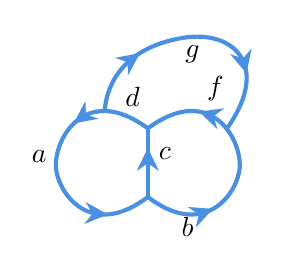
\begin{tikzpicture}[x=0.75pt,y=0.75pt,yscale=-1,xscale=1]
%uncomment if require: \path (0,106); %set diagram left start at 0, and has height of 106

%Straight Lines [id:da9297973117299008] 
\draw [color={rgb, 255:red, 74; green, 144; blue, 226 }  ,draw opacity=1 ][line width=1.5]    (334.08,48.63) -- (334.08,81.68) ;
\draw [shift={(334.08,58.06)}, rotate = 90] [fill={rgb, 255:red, 74; green, 144; blue, 226 }  ,fill opacity=1 ][line width=0.08]  [draw opacity=0] (11.07,-5.32) -- (0,0) -- (11.07,5.32) -- (7.35,0) -- cycle    ;
%Curve Lines [id:da05314264507602884] 
\draw [color={rgb, 255:red, 74; green, 144; blue, 226 }  ,draw opacity=1 ][line width=1.5]    (334.08,81.68) .. controls (308.75,101.02) and (292.63,82.97) .. (290.05,69.43) .. controls (287.48,55.89) and (302.95,25.6) .. (334.08,48.63) ;
\draw [shift={(314.77,90.07)}, rotate = 183.34] [fill={rgb, 255:red, 74; green, 144; blue, 226 }  ,fill opacity=1 ][line width=0.08]  [draw opacity=0] (11.07,-5.32) -- (0,0) -- (11.07,5.32) -- (7.35,0) -- cycle    ;
\draw [shift={(298.34,46.31)}, rotate = 323.19] [fill={rgb, 255:red, 74; green, 144; blue, 226 }  ,fill opacity=1 ][line width=0.08]  [draw opacity=0] (11.07,-5.32) -- (0,0) -- (11.07,5.32) -- (7.35,0) -- cycle    ;
%Curve Lines [id:da17723901531831388] 
\draw [color={rgb, 255:red, 74; green, 144; blue, 226 }  ,draw opacity=1 ][line width=1.5]    (334.08,81.68) .. controls (359.41,101.02) and (375.52,82.97) .. (378.1,69.43) .. controls (380.68,55.89) and (365.21,25.6) .. (334.08,48.63) ;
\draw [shift={(365.51,87.41)}, rotate = 158.56] [fill={rgb, 255:red, 74; green, 144; blue, 226 }  ,fill opacity=1 ][line width=0.08]  [draw opacity=0] (11.07,-5.32) -- (0,0) -- (11.07,5.32) -- (7.35,0) -- cycle    ;
\draw [shift={(358.76,40.55)}, rotate = 18.12] [fill={rgb, 255:red, 74; green, 144; blue, 226 }  ,fill opacity=1 ][line width=0.08]  [draw opacity=0] (11.07,-5.32) -- (0,0) -- (11.07,5.32) -- (7.35,0) -- cycle    ;
%Curve Lines [id:da9342861714656272] 
\draw [color={rgb, 255:red, 74; green, 144; blue, 226 }  ,draw opacity=1 ][line width=1.5]    (313.26,40.42) .. controls (314.55,23.02) and (326.8,8.84) .. (351.29,4.97) .. controls (375.78,1.11) and (393.19,18.51) .. (372.56,48.16) ;
\draw [shift={(330.26,12.37)}, rotate = 143.63] [fill={rgb, 255:red, 74; green, 144; blue, 226 }  ,fill opacity=1 ][line width=0.08]  [draw opacity=0] (11.07,-5.32) -- (0,0) -- (11.07,5.32) -- (7.35,0) -- cycle    ;
\draw [shift={(381.6,22.21)}, rotate = 255.76] [fill={rgb, 255:red, 74; green, 144; blue, 226 }  ,fill opacity=1 ][line width=0.08]  [draw opacity=0] (11.07,-5.32) -- (0,0) -- (11.07,5.32) -- (7.35,0) -- cycle    ;

% Text Node
\draw (348.88,89.98) node [anchor=north west][inner sep=0.75pt]    {$b$};
% Text Node
\draw (276.69,57.75) node [anchor=north west][inner sep=0.75pt]    {$a$};
% Text Node
\draw (337.93,56.46) node [anchor=north west][inner sep=0.75pt]    {$c$};
% Text Node
\draw (321.81,27.45) node [anchor=north west][inner sep=0.75pt]    {$d$};
% Text Node
\draw (361.13,21.87) node [anchor=north west][inner sep=0.75pt]    {$f$};
% Text Node
\draw (350.62,7.42) node [anchor=north west][inner sep=0.75pt]    {$g$};
\end{tikzpicture}
\end{figure}

\paragraph{Answer}

Direct computation gives:
\begin{align*}
\tikzset{every picture/.style={line width=0.75pt}} %set default line width to 0.75pt        
\begin{tikzpicture}[x=0.75pt,y=0.75pt,yscale=-1,xscale=1, baseline=(XXXX.south) ]
\path (0,105);\path (109.99577331542969,0);\draw    ($(current bounding box.center)+(0,0.3em)$) node [anchor=south] (XXXX) {};
%Straight Lines [id:da7121905477679571] 
\draw [color={rgb, 255:red, 74; green, 144; blue, 226 }  ,draw opacity=1 ][line width=0.75]    (57.95,48.66) -- (57.95,81.7) ;
\draw [shift={(57.95,59.88)}, rotate = 90] [fill={rgb, 255:red, 74; green, 144; blue, 226 }  ,fill opacity=1 ][line width=0.08]  [draw opacity=0] (8.93,-4.29) -- (0,0) -- (8.93,4.29) -- (5.93,0) -- cycle    ;
%Curve Lines [id:da6627190718130422] 
\draw [color={rgb, 255:red, 74; green, 144; blue, 226 }  ,draw opacity=1 ][line width=0.75]    (57.95,81.7) .. controls (32.62,101.04) and (16.5,82.99) .. (13.92,69.46) .. controls (11.35,55.92) and (26.82,25.62) .. (57.95,48.66) ;
\draw [shift={(36.89,90.16)}, rotate = 188.1] [fill={rgb, 255:red, 74; green, 144; blue, 226 }  ,fill opacity=1 ][line width=0.08]  [draw opacity=0] (8.93,-4.29) -- (0,0) -- (8.93,4.29) -- (5.93,0) -- cycle    ;
\draw [shift={(23.52,45.15)}, rotate = 327.89] [fill={rgb, 255:red, 74; green, 144; blue, 226 }  ,fill opacity=1 ][line width=0.08]  [draw opacity=0] (8.93,-4.29) -- (0,0) -- (8.93,4.29) -- (5.93,0) -- cycle    ;
%Curve Lines [id:da8374582275688303] 
\draw [color={rgb, 255:red, 74; green, 144; blue, 226 }  ,draw opacity=1 ][line width=0.75]    (57.95,81.7) .. controls (83.28,101.04) and (99.39,82.99) .. (101.97,69.46) .. controls (104.55,55.92) and (89.08,25.62) .. (57.95,48.66) ;
\draw [shift={(87.81,88.24)}, rotate = 163.53] [fill={rgb, 255:red, 74; green, 144; blue, 226 }  ,fill opacity=1 ][line width=0.08]  [draw opacity=0] (8.93,-4.29) -- (0,0) -- (8.93,4.29) -- (5.93,0) -- cycle    ;
\draw [shift={(84.48,40.98)}, rotate = 23.37] [fill={rgb, 255:red, 74; green, 144; blue, 226 }  ,fill opacity=1 ][line width=0.08]  [draw opacity=0] (8.93,-4.29) -- (0,0) -- (8.93,4.29) -- (5.93,0) -- cycle    ;
%Curve Lines [id:da7073273411206515] 
\draw [color={rgb, 255:red, 74; green, 144; blue, 226 }  ,draw opacity=1 ][line width=0.75]    (37.13,40.45) .. controls (38.42,23.05) and (50.67,8.86) .. (75.16,5) .. controls (99.65,1.13) and (118.2,20.59) .. (97.57,50.24) ;
\draw [shift={(52.47,13.48)}, rotate = 140.79] [fill={rgb, 255:red, 74; green, 144; blue, 226 }  ,fill opacity=1 ][line width=0.08]  [draw opacity=0] (8.93,-4.29) -- (0,0) -- (8.93,4.29) -- (5.93,0) -- cycle    ;
\draw [shift={(105.94,21.57)}, rotate = 249.52] [fill={rgb, 255:red, 74; green, 144; blue, 226 }  ,fill opacity=1 ][line width=0.08]  [draw opacity=0] (8.93,-4.29) -- (0,0) -- (8.93,4.29) -- (5.93,0) -- cycle    ;
% Text Node
\draw (72.75,88.5) node [anchor=north west][inner sep=0.75pt]    {$b$};
% Text Node
\draw (0.56,56.27) node [anchor=north west][inner sep=0.75pt]    {$a$};
% Text Node
\draw (61.8,54.98) node [anchor=north west][inner sep=0.75pt]    {$c$};
% Text Node
\draw (45.68,25.98) node [anchor=north west][inner sep=0.75pt]    {$d$};
% Text Node
\draw (86,21.4) node [anchor=north west][inner sep=0.75pt]    {$f$};
% Text Node
\draw (74.49,5.94) node [anchor=north west][inner sep=0.75pt]    {$g$};
\end{tikzpicture}
 & =\tikzset{every picture/.style={line width=0.75pt}} %set default line width to 0.75pt        
\begin{tikzpicture}[x=0.75pt,y=0.75pt,yscale=-1,xscale=1, baseline=(XXXX.south) ]
\path (0,87);\path (108.99190521240234,0);\draw    ($(current bounding box.center)+(0,0.3em)$) node [anchor=south] (XXXX) {};
%Straight Lines [id:da6909521486032779] 
\draw [color={rgb, 255:red, 74; green, 144; blue, 226 }  ,draw opacity=1 ]   (5,55) -- (35,85) ;
\draw [shift={(21.83,71.83)}, rotate = 225] [fill={rgb, 255:red, 74; green, 144; blue, 226 }  ,fill opacity=1 ][line width=0.08]  [draw opacity=0] (7.14,-3.43) -- (0,0) -- (7.14,3.43) -- (4.74,0) -- cycle    ;
%Straight Lines [id:da8409948327473487] 
\draw [color={rgb, 255:red, 74; green, 144; blue, 226 }  ,draw opacity=1 ]   (35,85) -- (55,65) ;
\draw [shift={(46.83,73.16)}, rotate = 135] [fill={rgb, 255:red, 74; green, 144; blue, 226 }  ,fill opacity=1 ][line width=0.08]  [draw opacity=0] (7.14,-3.43) -- (0,0) -- (7.14,3.43) -- (4.74,0) -- cycle    ;
%Straight Lines [id:da17445782339227334] 
\draw [color={rgb, 255:red, 74; green, 144; blue, 226 }  ,draw opacity=1 ]   (55,65) -- (75,85) ;
\draw [shift={(66.83,76.83)}, rotate = 225] [fill={rgb, 255:red, 74; green, 144; blue, 226 }  ,fill opacity=1 ][line width=0.08]  [draw opacity=0] (7.14,-3.43) -- (0,0) -- (7.14,3.43) -- (4.74,0) -- cycle    ;
%Straight Lines [id:da8723470143458258] 
\draw [color={rgb, 255:red, 74; green, 144; blue, 226 }  ,draw opacity=1 ]   (75,85) -- (105,55) ;
\draw [shift={(91.83,68.16)}, rotate = 135] [fill={rgb, 255:red, 74; green, 144; blue, 226 }  ,fill opacity=1 ][line width=0.08]  [draw opacity=0] (7.14,-3.43) -- (0,0) -- (7.14,3.43) -- (4.74,0) -- cycle    ;
%Straight Lines [id:da41858000719196387] 
\draw [color={rgb, 255:red, 74; green, 144; blue, 226 }  ,draw opacity=1 ]   (55,65) -- (55,45) ;
\draw [shift={(55,52.4)}, rotate = 90] [fill={rgb, 255:red, 74; green, 144; blue, 226 }  ,fill opacity=1 ][line width=0.08]  [draw opacity=0] (7.14,-3.43) -- (0,0) -- (7.14,3.43) -- (4.74,0) -- cycle    ;
%Straight Lines [id:da45912966223104124] 
\draw [color={rgb, 255:red, 74; green, 144; blue, 226 }  ,draw opacity=1 ]   (35,25) -- (5,55) ;
\draw [shift={(18.16,41.83)}, rotate = 315] [fill={rgb, 255:red, 74; green, 144; blue, 226 }  ,fill opacity=1 ][line width=0.08]  [draw opacity=0] (7.14,-3.43) -- (0,0) -- (7.14,3.43) -- (4.74,0) -- cycle    ;
%Straight Lines [id:da22416164342426503] 
\draw [color={rgb, 255:red, 74; green, 144; blue, 226 }  ,draw opacity=1 ]   (55,45) -- (35,25) ;
\draw [shift={(43.16,33.16)}, rotate = 45] [fill={rgb, 255:red, 74; green, 144; blue, 226 }  ,fill opacity=1 ][line width=0.08]  [draw opacity=0] (7.14,-3.43) -- (0,0) -- (7.14,3.43) -- (4.74,0) -- cycle    ;
%Straight Lines [id:da3205440188251567] 
\draw [color={rgb, 255:red, 74; green, 144; blue, 226 }  ,draw opacity=1 ]   (105,55) -- (75,25) ;
\draw [shift={(88.16,38.16)}, rotate = 45] [fill={rgb, 255:red, 74; green, 144; blue, 226 }  ,fill opacity=1 ][line width=0.08]  [draw opacity=0] (7.14,-3.43) -- (0,0) -- (7.14,3.43) -- (4.74,0) -- cycle    ;
%Straight Lines [id:da37140908300554343] 
\draw [color={rgb, 255:red, 74; green, 144; blue, 226 }  ,draw opacity=1 ]   (75,25) -- (55,45) ;
\draw [shift={(63.16,36.83)}, rotate = 315] [fill={rgb, 255:red, 74; green, 144; blue, 226 }  ,fill opacity=1 ][line width=0.08]  [draw opacity=0] (7.14,-3.43) -- (0,0) -- (7.14,3.43) -- (4.74,0) -- cycle    ;
%Straight Lines [id:da19782033550992173] 
\draw [color={rgb, 255:red, 74; green, 144; blue, 226 }  ,draw opacity=1 ]   (35,25) -- (55,5) ;
\draw [shift={(46.83,13.16)}, rotate = 135] [fill={rgb, 255:red, 74; green, 144; blue, 226 }  ,fill opacity=1 ][line width=0.08]  [draw opacity=0] (7.14,-3.43) -- (0,0) -- (7.14,3.43) -- (4.74,0) -- cycle    ;
%Straight Lines [id:da27846886728635356] 
\draw [color={rgb, 255:red, 74; green, 144; blue, 226 }  ,draw opacity=1 ]   (55,5) -- (75,25) ;
\draw [shift={(66.83,16.83)}, rotate = 225] [fill={rgb, 255:red, 74; green, 144; blue, 226 }  ,fill opacity=1 ][line width=0.08]  [draw opacity=0] (7.14,-3.43) -- (0,0) -- (7.14,3.43) -- (4.74,0) -- cycle    ;
% Text Node
\draw (3,67.5) node [anchor=north west][inner sep=0.75pt]    {$a$};
% Text Node
\draw (3,25.5) node [anchor=north west][inner sep=0.75pt]    {$a$};
% Text Node
\draw (33,55.5) node [anchor=north west][inner sep=0.75pt]    {$a$};
% Text Node
\draw (63,55.5) node [anchor=north west][inner sep=0.75pt]    {$b$};
% Text Node
\draw (92,71.5) node [anchor=north west][inner sep=0.75pt]    {$b$};
% Text Node
\draw (96,27.5) node [anchor=north west][inner sep=0.75pt]    {$b$};
% Text Node
\draw (44,44.5) node [anchor=north west][inner sep=0.75pt]    {$c$};
% Text Node
\draw (30,28.5) node [anchor=north west][inner sep=0.75pt]    {$d$};
% Text Node
\draw (66,30) node [anchor=north west][inner sep=0.75pt]    {$f$};
% Text Node
\draw (33,-2.5) node [anchor=north west][inner sep=0.75pt]    {$g$};
% Text Node
\draw (73,-2.5) node [anchor=north west][inner sep=0.75pt]    {$g$};
\end{tikzpicture}
=[F_{\overline{b}}^{a\overline{a}\overline{b}} ]_{Ic}\tikzset{every picture/.style={line width=0.75pt}} %set default line width to 0.75pt        
\begin{tikzpicture}[x=0.75pt,y=0.75pt,yscale=-1,xscale=1, baseline=(XXXX.south) ]
\path (0,87);\path (88.98342895507812,0);\draw    ($(current bounding box.center)+(0,0.3em)$) node [anchor=south] (XXXX) {};
%Straight Lines [id:da4268305986008065] 
\draw [color={rgb, 255:red, 74; green, 144; blue, 226 }  ,draw opacity=1 ]   (2.99,44.99) -- (22.99,64.99) ;
\draw [shift={(14.83,56.83)}, rotate = 225] [fill={rgb, 255:red, 74; green, 144; blue, 226 }  ,fill opacity=1 ][line width=0.08]  [draw opacity=0] (7.14,-3.43) -- (0,0) -- (7.14,3.43) -- (4.74,0) -- cycle    ;
%Straight Lines [id:da33618413816495485] 
\draw [color={rgb, 255:red, 74; green, 144; blue, 226 }  ,draw opacity=1 ]   (22.99,64.99) -- (42.99,84.99) ;
\draw [shift={(34.83,76.83)}, rotate = 225] [fill={rgb, 255:red, 74; green, 144; blue, 226 }  ,fill opacity=1 ][line width=0.08]  [draw opacity=0] (7.14,-3.43) -- (0,0) -- (7.14,3.43) -- (4.74,0) -- cycle    ;
%Straight Lines [id:da9515095691946336] 
\draw [color={rgb, 255:red, 74; green, 144; blue, 226 }  ,draw opacity=1 ]   (42.99,84.99) -- (82.99,44.99) ;
\draw [shift={(64.83,63.16)}, rotate = 135] [fill={rgb, 255:red, 74; green, 144; blue, 226 }  ,fill opacity=1 ][line width=0.08]  [draw opacity=0] (7.14,-3.43) -- (0,0) -- (7.14,3.43) -- (4.74,0) -- cycle    ;
%Straight Lines [id:da7154646006800551] 
\draw [color={rgb, 255:red, 74; green, 144; blue, 226 }  ,draw opacity=1 ]   (22.99,64.99) -- (42.99,44.99) ;
\draw [shift={(34.83,53.16)}, rotate = 135] [fill={rgb, 255:red, 74; green, 144; blue, 226 }  ,fill opacity=1 ][line width=0.08]  [draw opacity=0] (7.14,-3.43) -- (0,0) -- (7.14,3.43) -- (4.74,0) -- cycle    ;
%Straight Lines [id:da30070770172026906] 
\draw [color={rgb, 255:red, 74; green, 144; blue, 226 }  ,draw opacity=1 ]   (22.99,24.99) -- (2.99,44.99) ;
\draw [shift={(11.15,36.83)}, rotate = 315] [fill={rgb, 255:red, 74; green, 144; blue, 226 }  ,fill opacity=1 ][line width=0.08]  [draw opacity=0] (7.14,-3.43) -- (0,0) -- (7.14,3.43) -- (4.74,0) -- cycle    ;
%Straight Lines [id:da6403009110238249] 
\draw [color={rgb, 255:red, 74; green, 144; blue, 226 }  ,draw opacity=1 ]   (42.99,44.99) -- (22.99,24.99) ;
\draw [shift={(31.15,33.16)}, rotate = 45] [fill={rgb, 255:red, 74; green, 144; blue, 226 }  ,fill opacity=1 ][line width=0.08]  [draw opacity=0] (7.14,-3.43) -- (0,0) -- (7.14,3.43) -- (4.74,0) -- cycle    ;
%Straight Lines [id:da03682326082461018] 
\draw [color={rgb, 255:red, 74; green, 144; blue, 226 }  ,draw opacity=1 ]   (82.99,44.99) -- (62.99,24.99) ;
\draw [shift={(71.15,33.16)}, rotate = 45] [fill={rgb, 255:red, 74; green, 144; blue, 226 }  ,fill opacity=1 ][line width=0.08]  [draw opacity=0] (7.14,-3.43) -- (0,0) -- (7.14,3.43) -- (4.74,0) -- cycle    ;
%Straight Lines [id:da1950534113724205] 
\draw [color={rgb, 255:red, 74; green, 144; blue, 226 }  ,draw opacity=1 ]   (62.99,24.99) -- (42.99,44.99) ;
\draw [shift={(51.15,36.83)}, rotate = 315] [fill={rgb, 255:red, 74; green, 144; blue, 226 }  ,fill opacity=1 ][line width=0.08]  [draw opacity=0] (7.14,-3.43) -- (0,0) -- (7.14,3.43) -- (4.74,0) -- cycle    ;
%Straight Lines [id:da23314488082045193] 
\draw [color={rgb, 255:red, 74; green, 144; blue, 226 }  ,draw opacity=1 ]   (22.99,24.99) -- (42.99,4.99) ;
\draw [shift={(34.83,13.16)}, rotate = 135] [fill={rgb, 255:red, 74; green, 144; blue, 226 }  ,fill opacity=1 ][line width=0.08]  [draw opacity=0] (7.14,-3.43) -- (0,0) -- (7.14,3.43) -- (4.74,0) -- cycle    ;
%Straight Lines [id:da19644739853176252] 
\draw [color={rgb, 255:red, 74; green, 144; blue, 226 }  ,draw opacity=1 ]   (42.99,4.99) -- (62.99,24.99) ;
\draw [shift={(54.83,16.83)}, rotate = 225] [fill={rgb, 255:red, 74; green, 144; blue, 226 }  ,fill opacity=1 ][line width=0.08]  [draw opacity=0] (7.14,-3.43) -- (0,0) -- (7.14,3.43) -- (4.74,0) -- cycle    ;
% Text Node
\draw (0,52) node [anchor=north west][inner sep=0.75pt]    {$a$};
% Text Node
\draw (0.99,17.49) node [anchor=north west][inner sep=0.75pt]    {$a$};
% Text Node
\draw (14.99,71.49) node [anchor=north west][inner sep=0.75pt]    {$b$};
% Text Node
\draw (59.99,71.49) node [anchor=north west][inner sep=0.75pt]    {$b$};
% Text Node
\draw (33.99,52) node [anchor=north west][inner sep=0.75pt]    {$c$};
% Text Node
\draw (21.99,35) node [anchor=north west][inner sep=0.75pt]    {$d$};
% Text Node
\draw (53.99,31.49) node [anchor=north west][inner sep=0.75pt]    {$f$};
% Text Node
\draw (20.99,-4.51) node [anchor=north west][inner sep=0.75pt]    {$g$};
% Text Node
\draw (53.99,-4.51) node [anchor=north west][inner sep=0.75pt]    {$g$};
% Text Node
\draw (71.99,19.49) node [anchor=north west][inner sep=0.75pt]    {$b$};
\end{tikzpicture}
\\
 & =[F_{\overline{b}}^{a\overline{a}\overline{b}} ]_{Ic} [F_{I}^{\overline{b} f\overline{g}} ]_{gb}\tikzset{every picture/.style={line width=0.75pt}} %set default line width to 0.75pt        
\begin{tikzpicture}[x=0.75pt,y=0.75pt,yscale=-1,xscale=1, baseline=(XXXX.south) ]
\path (0,95);\path (88.98342895507812,0);\draw    ($(current bounding box.center)+(0,0.3em)$) node [anchor=south] (XXXX) {};
%Straight Lines [id:da8395138178233774] 
\draw [color={rgb, 255:red, 74; green, 144; blue, 226 }  ,draw opacity=1 ]   (4.98,48.99) -- (24.98,68.99) ;
\draw [shift={(16.82,60.83)}, rotate = 225] [fill={rgb, 255:red, 74; green, 144; blue, 226 }  ,fill opacity=1 ][line width=0.08]  [draw opacity=0] (7.14,-3.43) -- (0,0) -- (7.14,3.43) -- (4.74,0) -- cycle    ;
%Straight Lines [id:da7657469873325047] 
\draw [color={rgb, 255:red, 74; green, 144; blue, 226 }  ,draw opacity=1 ]   (24.98,68.99) -- (44.98,88.99) ;
\draw [shift={(36.82,80.83)}, rotate = 225] [fill={rgb, 255:red, 74; green, 144; blue, 226 }  ,fill opacity=1 ][line width=0.08]  [draw opacity=0] (7.14,-3.43) -- (0,0) -- (7.14,3.43) -- (4.74,0) -- cycle    ;
%Straight Lines [id:da4877396143003214] 
\draw [color={rgb, 255:red, 74; green, 144; blue, 226 }  ,draw opacity=1 ]   (44.98,88.99) -- (84.98,48.99) ;
\draw [shift={(66.82,67.16)}, rotate = 135] [fill={rgb, 255:red, 74; green, 144; blue, 226 }  ,fill opacity=1 ][line width=0.08]  [draw opacity=0] (7.14,-3.43) -- (0,0) -- (7.14,3.43) -- (4.74,0) -- cycle    ;
%Straight Lines [id:da1272150987243279] 
\draw [color={rgb, 255:red, 74; green, 144; blue, 226 }  ,draw opacity=1 ]   (24.98,68.99) -- (44.98,48.99) ;
\draw [shift={(36.82,57.16)}, rotate = 135] [fill={rgb, 255:red, 74; green, 144; blue, 226 }  ,fill opacity=1 ][line width=0.08]  [draw opacity=0] (7.14,-3.43) -- (0,0) -- (7.14,3.43) -- (4.74,0) -- cycle    ;
%Straight Lines [id:da10415354691994083] 
\draw [color={rgb, 255:red, 74; green, 144; blue, 226 }  ,draw opacity=1 ]   (24.98,28.99) -- (4.98,48.99) ;
\draw [shift={(13.14,40.83)}, rotate = 315] [fill={rgb, 255:red, 74; green, 144; blue, 226 }  ,fill opacity=1 ][line width=0.08]  [draw opacity=0] (7.14,-3.43) -- (0,0) -- (7.14,3.43) -- (4.74,0) -- cycle    ;
%Straight Lines [id:da3069166424268277] 
\draw [color={rgb, 255:red, 74; green, 144; blue, 226 }  ,draw opacity=1 ]   (44.98,48.99) -- (24.98,28.99) ;
\draw [shift={(33.14,37.16)}, rotate = 45] [fill={rgb, 255:red, 74; green, 144; blue, 226 }  ,fill opacity=1 ][line width=0.08]  [draw opacity=0] (7.14,-3.43) -- (0,0) -- (7.14,3.43) -- (4.74,0) -- cycle    ;
%Straight Lines [id:da5800008857317709] 
\draw [color={rgb, 255:red, 74; green, 144; blue, 226 }  ,draw opacity=1 ]   (84.98,48.99) -- (44.98,8.99) ;
\draw [shift={(63.14,27.16)}, rotate = 45] [fill={rgb, 255:red, 74; green, 144; blue, 226 }  ,fill opacity=1 ][line width=0.08]  [draw opacity=0] (7.14,-3.43) -- (0,0) -- (7.14,3.43) -- (4.74,0) -- cycle    ;
%Straight Lines [id:da4219457762886294] 
\draw [color={rgb, 255:red, 74; green, 144; blue, 226 }  ,draw opacity=1 ]   (34.98,18.99) -- (44.98,48.99) ;
\draw [shift={(40.81,36.46)}, rotate = 251.57] [fill={rgb, 255:red, 74; green, 144; blue, 226 }  ,fill opacity=1 ][line width=0.08]  [draw opacity=0] (7.14,-3.43) -- (0,0) -- (7.14,3.43) -- (4.74,0) -- cycle    ;
%Straight Lines [id:da8413650016839056] 
\draw [color={rgb, 255:red, 74; green, 144; blue, 226 }  ,draw opacity=1 ]   (24.98,28.99) -- (34.98,18.99) ;
\draw [shift={(31.82,22.16)}, rotate = 135] [fill={rgb, 255:red, 74; green, 144; blue, 226 }  ,fill opacity=1 ][line width=0.08]  [draw opacity=0] (7.14,-3.43) -- (0,0) -- (7.14,3.43) -- (4.74,0) -- cycle    ;
%Straight Lines [id:da5181256829613317] 
\draw [color={rgb, 255:red, 74; green, 144; blue, 226 }  ,draw opacity=1 ]   (44.98,8.99) -- (34.98,18.99) ;
\draw [shift={(38.14,15.83)}, rotate = 315] [fill={rgb, 255:red, 74; green, 144; blue, 226 }  ,fill opacity=1 ][line width=0.08]  [draw opacity=0] (7.14,-3.43) -- (0,0) -- (7.14,3.43) -- (4.74,0) -- cycle    ;
% Text Node
\draw (0,57) node [anchor=north west][inner sep=0.75pt]    {$a$};
% Text Node
\draw (2.98,21.49) node [anchor=north west][inner sep=0.75pt]    {$a$};
% Text Node
\draw (16.98,75.49) node [anchor=north west][inner sep=0.75pt]    {$b$};
% Text Node
\draw (61.98,75.49) node [anchor=north west][inner sep=0.75pt]    {$b$};
% Text Node
\draw (35.98,57) node [anchor=north west][inner sep=0.75pt]    {$c$};
% Text Node
\draw (23.98,39) node [anchor=north west][inner sep=0.75pt]    {$d$};
% Text Node
\draw (42.98,21.49) node [anchor=north west][inner sep=0.75pt]    {$f$};
% Text Node
\draw (18.98,7.49) node [anchor=north west][inner sep=0.75pt]    {$g$};
% Text Node
\draw (55.98,1.49) node [anchor=north west][inner sep=0.75pt]    {$b$};
% Text Node
\draw (27.98,-0.51) node [anchor=north west][inner sep=0.75pt]    {$b$};
\end{tikzpicture}
\\
 & =[F_{\overline{b}}^{a\overline{a}\overline{b}} ]_{Ic} [F_{I}^{\overline{b} f\overline{g}} ]_{gb} [F_{\overline{b}}^{\overline{a} d\overline{f}} ]_{cg}^{*}\tikzset{every picture/.style={line width=0.75pt}} %set default line width to 0.75pt        
\begin{tikzpicture}[x=0.75pt,y=0.75pt,yscale=-1,xscale=1, baseline=(XXXX.south) ]
\path (0,92);\path (88.98342895507812,0);\draw    ($(current bounding box.center)+(0,0.3em)$) node [anchor=south] (XXXX) {};
%Straight Lines [id:da3810427737406432] 
\draw [color={rgb, 255:red, 74; green, 144; blue, 226 }  ,draw opacity=1 ]   (8.98,46.99) -- (18.98,56.99) ;
\draw [shift={(15.82,53.82)}, rotate = 225] [fill={rgb, 255:red, 74; green, 144; blue, 226 }  ,fill opacity=1 ][line width=0.08]  [draw opacity=0] (7.14,-3.43) -- (0,0) -- (7.14,3.43) -- (4.74,0) -- cycle    ;
%Straight Lines [id:da5616521968042418] 
\draw [color={rgb, 255:red, 74; green, 144; blue, 226 }  ,draw opacity=1 ]   (28.98,66.99) -- (48.98,86.99) ;
\draw [shift={(40.82,78.82)}, rotate = 225] [fill={rgb, 255:red, 74; green, 144; blue, 226 }  ,fill opacity=1 ][line width=0.08]  [draw opacity=0] (7.14,-3.43) -- (0,0) -- (7.14,3.43) -- (4.74,0) -- cycle    ;
%Straight Lines [id:da05018316330971162] 
\draw [color={rgb, 255:red, 74; green, 144; blue, 226 }  ,draw opacity=1 ]   (48.98,86.99) -- (88.98,46.99) ;
\draw [shift={(70.82,65.15)}, rotate = 135] [fill={rgb, 255:red, 74; green, 144; blue, 226 }  ,fill opacity=1 ][line width=0.08]  [draw opacity=0] (7.14,-3.43) -- (0,0) -- (7.14,3.43) -- (4.74,0) -- cycle    ;
%Straight Lines [id:da19897361937741964] 
\draw [color={rgb, 255:red, 74; green, 144; blue, 226 }  ,draw opacity=1 ]   (28.98,66.99) -- (48.98,46.99) ;
\draw [shift={(40.82,55.15)}, rotate = 135] [fill={rgb, 255:red, 74; green, 144; blue, 226 }  ,fill opacity=1 ][line width=0.08]  [draw opacity=0] (7.14,-3.43) -- (0,0) -- (7.14,3.43) -- (4.74,0) -- cycle    ;
%Straight Lines [id:da6787672731817094] 
\draw [color={rgb, 255:red, 74; green, 144; blue, 226 }  ,draw opacity=1 ]   (28.98,26.99) -- (8.98,46.99) ;
\draw [shift={(17.14,38.82)}, rotate = 315] [fill={rgb, 255:red, 74; green, 144; blue, 226 }  ,fill opacity=1 ][line width=0.08]  [draw opacity=0] (7.14,-3.43) -- (0,0) -- (7.14,3.43) -- (4.74,0) -- cycle    ;
%Straight Lines [id:da6143001329307365] 
\draw [color={rgb, 255:red, 74; green, 144; blue, 226 }  ,draw opacity=1 ]   (18.98,56.99) -- (28.98,26.99) ;
\draw [shift={(24.81,39.52)}, rotate = 108.43] [fill={rgb, 255:red, 74; green, 144; blue, 226 }  ,fill opacity=1 ][line width=0.08]  [draw opacity=0] (7.14,-3.43) -- (0,0) -- (7.14,3.43) -- (4.74,0) -- cycle    ;
%Straight Lines [id:da8634871158502804] 
\draw [color={rgb, 255:red, 74; green, 144; blue, 226 }  ,draw opacity=1 ]   (88.98,46.99) -- (48.98,6.99) ;
\draw [shift={(67.14,25.15)}, rotate = 45] [fill={rgb, 255:red, 74; green, 144; blue, 226 }  ,fill opacity=1 ][line width=0.08]  [draw opacity=0] (7.14,-3.43) -- (0,0) -- (7.14,3.43) -- (4.74,0) -- cycle    ;
%Straight Lines [id:da1328317384738471] 
\draw [color={rgb, 255:red, 74; green, 144; blue, 226 }  ,draw opacity=1 ]   (38.98,16.99) -- (48.98,46.99) ;
\draw [shift={(44.81,34.45)}, rotate = 251.57] [fill={rgb, 255:red, 74; green, 144; blue, 226 }  ,fill opacity=1 ][line width=0.08]  [draw opacity=0] (7.14,-3.43) -- (0,0) -- (7.14,3.43) -- (4.74,0) -- cycle    ;
%Straight Lines [id:da4586185861340333] 
\draw [color={rgb, 255:red, 74; green, 144; blue, 226 }  ,draw opacity=1 ]   (28.98,26.99) -- (38.98,16.99) ;
\draw [shift={(35.82,20.15)}, rotate = 135] [fill={rgb, 255:red, 74; green, 144; blue, 226 }  ,fill opacity=1 ][line width=0.08]  [draw opacity=0] (7.14,-3.43) -- (0,0) -- (7.14,3.43) -- (4.74,0) -- cycle    ;
%Straight Lines [id:da41754427438218045] 
\draw [color={rgb, 255:red, 74; green, 144; blue, 226 }  ,draw opacity=1 ]   (48.98,6.99) -- (38.98,16.99) ;
\draw [shift={(42.14,13.82)}, rotate = 315] [fill={rgb, 255:red, 74; green, 144; blue, 226 }  ,fill opacity=1 ][line width=0.08]  [draw opacity=0] (7.14,-3.43) -- (0,0) -- (7.14,3.43) -- (4.74,0) -- cycle    ;
%Straight Lines [id:da05147982511322313] 
\draw [color={rgb, 255:red, 74; green, 144; blue, 226 }  ,draw opacity=1 ]   (18.98,56.99) -- (28.98,66.99) ;
\draw [shift={(25.82,63.82)}, rotate = 225] [fill={rgb, 255:red, 74; green, 144; blue, 226 }  ,fill opacity=1 ][line width=0.08]  [draw opacity=0] (7.14,-3.43) -- (0,0) -- (7.14,3.43) -- (4.74,0) -- cycle    ;
% Text Node
\draw (2.84,52) node [anchor=north west][inner sep=0.75pt]    {$a$};
% Text Node
\draw (6.98,19.49) node [anchor=north west][inner sep=0.75pt]    {$a$};
% Text Node
\draw (26.98,73.49) node [anchor=north west][inner sep=0.75pt]    {$b$};
% Text Node
\draw (63.98,70.49) node [anchor=north west][inner sep=0.75pt]    {$b$};
% Text Node
\draw (39.98,49.49) node [anchor=north west][inner sep=0.75pt]    {$f$};
% Text Node
\draw (27.98,32.49) node [anchor=north west][inner sep=0.75pt]    {$d$};
% Text Node
\draw (45.98,19.49) node [anchor=north west][inner sep=0.75pt]    {$f$};
% Text Node
\draw (22.98,5.49) node [anchor=north west][inner sep=0.75pt]    {$g$};
% Text Node
\draw (59.98,-0.51) node [anchor=north west][inner sep=0.75pt]    {$b$};
% Text Node
\draw (31.98,-2.51) node [anchor=north west][inner sep=0.75pt]    {$b$};
% Text Node
\draw (15.98,67) node [anchor=north west][inner sep=0.75pt]  [color={rgb, 255:red, 0; green, 0; blue, 0 }  ,opacity=1 ]  {$g$};
\end{tikzpicture}
\\
 & =[F_{\overline{b}}^{a\overline{a}\overline{b}} ]_{Ic} [F_{I}^{\overline{b} f\overline{g}} ]_{gb} [F_{\overline{b}}^{\overline{a} d\overline{f}} ]_{cg}^{*} .
\end{align*}

\section{Locality Principle}
Show that the locality principle (Fig.\ref{fig:noTransmutationPrinciple}) is derivable from our other rules for evaluating diagrams, and is not therefore an independent assumption.
\begin{figure}[h!]
\centering
\tikzset{every picture/.style={line width=0.75pt}} %set default line width to 0.75pt        

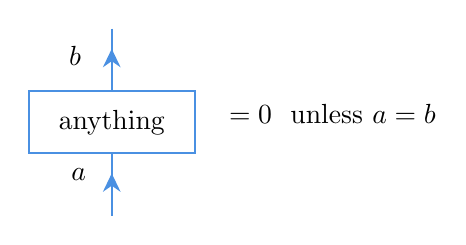
\begin{tikzpicture}[x=0.75pt,y=0.75pt,yscale=-1,xscale=1]
%uncomment if require: \path (0,96); %set diagram left start at 0, and has height of 96

%Straight Lines [id:da3911550496418774] 
\draw [color={rgb, 255:red, 74; green, 144; blue, 226 }  ,draw opacity=1 ][line width=0.75]    (267,63) -- (267,93) ;
\draw [shift={(267,72.7)}, rotate = 90] [fill={rgb, 255:red, 74; green, 144; blue, 226 }  ,fill opacity=1 ][line width=0.08]  [draw opacity=0] (8.93,-4.29) -- (0,0) -- (8.93,4.29) -- (5.93,0) -- cycle    ;
%Shape: Rectangle [id:dp4343028329905816] 
\draw  [color={rgb, 255:red, 74; green, 144; blue, 226 }  ,draw opacity=1 ] (227,33) -- (307,33) -- (307,63) -- (227,63) -- cycle ;
%Straight Lines [id:da2744694274843744] 
\draw [color={rgb, 255:red, 74; green, 144; blue, 226 }  ,draw opacity=1 ][line width=0.75]    (267,3) -- (267,33) ;
\draw [shift={(267,12.7)}, rotate = 90] [fill={rgb, 255:red, 74; green, 144; blue, 226 }  ,fill opacity=1 ][line width=0.08]  [draw opacity=0] (8.93,-4.29) -- (0,0) -- (8.93,4.29) -- (5.93,0) -- cycle    ;

% Text Node
\draw (267,48) node   [align=left] {anything};
% Text Node
\draw (246,69) node [anchor=north west][inner sep=0.75pt]    {$a$};
% Text Node
\draw (245,10) node [anchor=north west][inner sep=0.75pt]    {$b$};
% Text Node
\draw (322,38) node [anchor=north west][inner sep=0.75pt]   [align=left] {$=0$ \ unless $a=b$};
\end{tikzpicture}
\caption{The locality, or no-transmutation, principle as in Fig. 8.7.}
\label{fig:noTransmutationPrinciple}
\end{figure}

\paragraph{Answer}

Proof scheme: change every diagram into the standard basis, and use the orthogonality of the tree, such as the Eq. \eqref{eq:PlanarDiagramOrthogonality} below:
\begin{equation}
\tikzset{every picture/.style={line width=0.75pt}} %set default line width to 0.75pt        
\begin{tikzpicture}[x=0.75pt,y=0.75pt,yscale=-1,xscale=1, baseline=(XXXX.south) ]
\path (0,127);\path (100,0);\draw    ($(current bounding box.center)+(0,0.3em)$) node [anchor=south] (XXXX) {};
%Straight Lines [id:da6583219559913778] 
\draw [color={rgb, 255:red, 74; green, 144; blue, 226 }  ,draw opacity=1 ]   (50,106) -- (70,126) ;
\draw [shift={(57.1,113.1)}, rotate = 45] [fill={rgb, 255:red, 74; green, 144; blue, 226 }  ,fill opacity=1 ][line width=0.08]  [draw opacity=0] (7.14,-3.43) -- (0,0) -- (7.14,3.43) -- (4.74,0) -- cycle    ;
%Straight Lines [id:da2706825487108864] 
\draw [color={rgb, 255:red, 74; green, 144; blue, 226 }  ,draw opacity=1 ]   (30,86) -- (50,106) ;
\draw [shift={(37.1,93.1)}, rotate = 45] [fill={rgb, 255:red, 74; green, 144; blue, 226 }  ,fill opacity=1 ][line width=0.08]  [draw opacity=0] (7.14,-3.43) -- (0,0) -- (7.14,3.43) -- (4.74,0) -- cycle    ;
%Straight Lines [id:da6617340169244292] 
\draw [color={rgb, 255:red, 74; green, 144; blue, 226 }  ,draw opacity=1 ]   (10,66) -- (30,86) ;
\draw [shift={(17.1,73.1)}, rotate = 45] [fill={rgb, 255:red, 74; green, 144; blue, 226 }  ,fill opacity=1 ][line width=0.08]  [draw opacity=0] (7.14,-3.43) -- (0,0) -- (7.14,3.43) -- (4.74,0) -- cycle    ;
%Straight Lines [id:da18706855355386143] 
\draw [color={rgb, 255:red, 74; green, 144; blue, 226 }  ,draw opacity=1 ]   (50,66) -- (30,86) ;
\draw [shift={(42.9,73.1)}, rotate = 135] [fill={rgb, 255:red, 74; green, 144; blue, 226 }  ,fill opacity=1 ][line width=0.08]  [draw opacity=0] (7.14,-3.43) -- (0,0) -- (7.14,3.43) -- (4.74,0) -- cycle    ;
%Straight Lines [id:da6542059341419844] 
\draw [color={rgb, 255:red, 74; green, 144; blue, 226 }  ,draw opacity=1 ]   (90,66) -- (50,106) ;
\draw [shift={(72.9,83.1)}, rotate = 135] [fill={rgb, 255:red, 74; green, 144; blue, 226 }  ,fill opacity=1 ][line width=0.08]  [draw opacity=0] (7.14,-3.43) -- (0,0) -- (7.14,3.43) -- (4.74,0) -- cycle    ;
%Straight Lines [id:da5187159834083965] 
\draw [color={rgb, 255:red, 74; green, 144; blue, 226 }  ,draw opacity=1 ]   (50,26) -- (70,6) ;
\draw [shift={(61.84,14.16)}, rotate = 135] [fill={rgb, 255:red, 74; green, 144; blue, 226 }  ,fill opacity=1 ][line width=0.08]  [draw opacity=0] (7.14,-3.43) -- (0,0) -- (7.14,3.43) -- (4.74,0) -- cycle    ;
%Straight Lines [id:da2819710278996115] 
\draw [color={rgb, 255:red, 74; green, 144; blue, 226 }  ,draw opacity=1 ]   (30,46) -- (50,26) ;
\draw [shift={(41.84,34.16)}, rotate = 135] [fill={rgb, 255:red, 74; green, 144; blue, 226 }  ,fill opacity=1 ][line width=0.08]  [draw opacity=0] (7.14,-3.43) -- (0,0) -- (7.14,3.43) -- (4.74,0) -- cycle    ;
%Straight Lines [id:da09888241705981926] 
\draw [color={rgb, 255:red, 74; green, 144; blue, 226 }  ,draw opacity=1 ]   (10,66) -- (30,46) ;
\draw [shift={(21.84,54.16)}, rotate = 135] [fill={rgb, 255:red, 74; green, 144; blue, 226 }  ,fill opacity=1 ][line width=0.08]  [draw opacity=0] (7.14,-3.43) -- (0,0) -- (7.14,3.43) -- (4.74,0) -- cycle    ;
%Straight Lines [id:da5104207786896238] 
\draw [color={rgb, 255:red, 74; green, 144; blue, 226 }  ,draw opacity=1 ]   (50,66) -- (30,46) ;
\draw [shift={(38.16,54.16)}, rotate = 45] [fill={rgb, 255:red, 74; green, 144; blue, 226 }  ,fill opacity=1 ][line width=0.08]  [draw opacity=0] (7.14,-3.43) -- (0,0) -- (7.14,3.43) -- (4.74,0) -- cycle    ;
%Straight Lines [id:da09676188381782547] 
\draw [color={rgb, 255:red, 74; green, 144; blue, 226 }  ,draw opacity=1 ]   (90,66) -- (50,26) ;
\draw [shift={(68.16,44.16)}, rotate = 45] [fill={rgb, 255:red, 74; green, 144; blue, 226 }  ,fill opacity=1 ][line width=0.08]  [draw opacity=0] (7.14,-3.43) -- (0,0) -- (7.14,3.43) -- (4.74,0) -- cycle    ;
% Text Node
\draw (1,68.5) node [anchor=north west][inner sep=0.75pt]    {$a$};
% Text Node
\draw (48,68.5) node [anchor=north west][inner sep=0.75pt]    {$b$};
% Text Node
\draw (88,68.5) node [anchor=north west][inner sep=0.75pt]    {$c$};
% Text Node
\draw (21,88.5) node [anchor=north west][inner sep=0.75pt]    {$d$};
% Text Node
\draw (41,108.5) node [anchor=north west][inner sep=0.75pt]    {$e$};
% Text Node
\draw (1,48.5) node [anchor=north west][inner sep=0.75pt]    {$a'$};
% Text Node
\draw (48,48.5) node [anchor=north west][inner sep=0.75pt]    {$b'$};
% Text Node
\draw (88,48.5) node [anchor=north west][inner sep=0.75pt]    {$c'$};
% Text Node
\draw (21,18.5) node [anchor=north west][inner sep=0.75pt]    {$d'$};
% Text Node
\draw (48,-1.5) node [anchor=north west][inner sep=0.75pt]    {$e'$};
\end{tikzpicture}
=\delta _{aa'} \delta _{bb'} \delta _{cc'} \delta _{dd'} \delta _{ee'}\tikzset{every picture/.style={line width=0.75pt}} %set default line width to 0.75pt        
\begin{tikzpicture}[x=0.75pt,y=0.75pt,yscale=-1,xscale=1, baseline=(XXXX.south) ]
\path (0,108);\path (18.991836547851562,0);\draw    ($(current bounding box.center)+(0,0.3em)$) node [anchor=south] (XXXX) {};
%Straight Lines [id:da23811147262781374] 
\draw [color={rgb, 255:red, 74; green, 144; blue, 226 }  ,draw opacity=1 ]   (4,4) -- (4,105.51) ;
\draw [shift={(4,50.66)}, rotate = 90] [fill={rgb, 255:red, 74; green, 144; blue, 226 }  ,fill opacity=1 ][line width=0.08]  [draw opacity=0] (7.14,-3.43) -- (0,0) -- (7.14,3.43) -- (4.74,0) -- cycle    ;
% Text Node
\draw (8,47.5) node [anchor=north west][inner sep=0.75pt]    {$e$};
\end{tikzpicture}
.
\label{eq:PlanarDiagramOrthogonality}
\end{equation}
Firstly, we notice that the planar diagram must have the property that each vertex can only be linked to three edges at most, because we don't allow three anyons fusion at the same time, such as $a\times b\times c=d$. After changing it into standard basis, we can use the orthogonality relation to eliminate the bubbles. The algorithm of changing into standard basis is as follows:
\begin{enumerate}
\item  Start from the incoming anyon.
\item  Travel along the right line at the bottom
\item  For every following vertex, choose the right path, and use the basis changing to eliminate the left path
\item  Reach the outcoming anyon finally
\item  Travel along the left path from the last crossing which we haven't chosen the left path
\item  Repeat (c) to (e) for every vertex until every vertex in the diagram is traversed.
\end{enumerate}

We will look at several examples. Firstly, if $\boxed{\text{anything}}$ is planar diagram $K_{4}$ or butterfly graph as the Fig.\ref{fig:K4Butterfly} below shows, this is not allowed, because every vertex in $K_{4}$ are linked to three edges, and there is four-valent vertex in the butterfly graph. 

\begin{figure}[h!]
\centering
\tikzset{every picture/.style={line width=0.75pt}} %set default line width to 0.75pt        

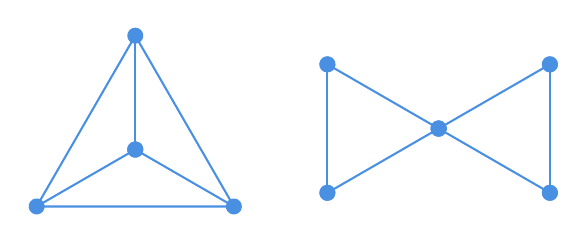
\begin{tikzpicture}[x=0.75pt,y=0.75pt,yscale=-1,xscale=1]
%uncomment if require: \path (0,95); %set diagram left start at 0, and has height of 95

%Shape: Regular Polygon [id:dp5227769047389439] 
\draw  [color={rgb, 255:red, 74; green, 144; blue, 226 }  ,draw opacity=1 ] (318.44,88.22) -- (223.42,88.22) -- (270.93,5.93) -- cycle ;
%Straight Lines [id:da03476734995525277] 
\draw [color={rgb, 255:red, 74; green, 144; blue, 226 }  ,draw opacity=1 ]   (270.93,60.79) -- (270.93,5.93) ;
\draw [shift={(270.93,5.93)}, rotate = 270] [color={rgb, 255:red, 74; green, 144; blue, 226 }  ,draw opacity=1 ][fill={rgb, 255:red, 74; green, 144; blue, 226 }  ,fill opacity=1 ][line width=0.75]      (0, 0) circle [x radius= 3.35, y radius= 3.35]   ;
\draw [shift={(270.93,60.79)}, rotate = 270] [color={rgb, 255:red, 74; green, 144; blue, 226 }  ,draw opacity=1 ][fill={rgb, 255:red, 74; green, 144; blue, 226 }  ,fill opacity=1 ][line width=0.75]      (0, 0) circle [x radius= 3.35, y radius= 3.35]   ;
%Straight Lines [id:da772600873513491] 
\draw [color={rgb, 255:red, 74; green, 144; blue, 226 }  ,draw opacity=1 ]   (270.93,60.79) -- (318.44,88.22) ;
\draw [shift={(318.44,88.22)}, rotate = 30] [color={rgb, 255:red, 74; green, 144; blue, 226 }  ,draw opacity=1 ][fill={rgb, 255:red, 74; green, 144; blue, 226 }  ,fill opacity=1 ][line width=0.75]      (0, 0) circle [x radius= 3.35, y radius= 3.35]   ;
\draw [shift={(270.93,60.79)}, rotate = 30] [color={rgb, 255:red, 74; green, 144; blue, 226 }  ,draw opacity=1 ][fill={rgb, 255:red, 74; green, 144; blue, 226 }  ,fill opacity=1 ][line width=0.75]      (0, 0) circle [x radius= 3.35, y radius= 3.35]   ;
%Straight Lines [id:da6349296820582229] 
\draw [color={rgb, 255:red, 74; green, 144; blue, 226 }  ,draw opacity=1 ]   (270.93,60.79) -- (223.42,88.22) ;
\draw [shift={(223.42,88.22)}, rotate = 150] [color={rgb, 255:red, 74; green, 144; blue, 226 }  ,draw opacity=1 ][fill={rgb, 255:red, 74; green, 144; blue, 226 }  ,fill opacity=1 ][line width=0.75]      (0, 0) circle [x radius= 3.35, y radius= 3.35]   ;
\draw [shift={(270.93,60.79)}, rotate = 150] [color={rgb, 255:red, 74; green, 144; blue, 226 }  ,draw opacity=1 ][fill={rgb, 255:red, 74; green, 144; blue, 226 }  ,fill opacity=1 ][line width=0.75]      (0, 0) circle [x radius= 3.35, y radius= 3.35]   ;
%Straight Lines [id:da41429372320099245] 
\draw [color={rgb, 255:red, 74; green, 144; blue, 226 }  ,draw opacity=1 ]   (363.5,81.64) -- (363.5,19.75) ;
\draw [shift={(363.5,19.75)}, rotate = 270] [color={rgb, 255:red, 74; green, 144; blue, 226 }  ,draw opacity=1 ][fill={rgb, 255:red, 74; green, 144; blue, 226 }  ,fill opacity=1 ][line width=0.75]      (0, 0) circle [x radius= 3.35, y radius= 3.35]   ;
\draw [shift={(363.5,81.64)}, rotate = 270] [color={rgb, 255:red, 74; green, 144; blue, 226 }  ,draw opacity=1 ][fill={rgb, 255:red, 74; green, 144; blue, 226 }  ,fill opacity=1 ][line width=0.75]      (0, 0) circle [x radius= 3.35, y radius= 3.35]   ;
%Straight Lines [id:da32758191647462853] 
\draw [color={rgb, 255:red, 74; green, 144; blue, 226 }  ,draw opacity=1 ]   (363.5,81.64) -- (417.1,50.69) ;
\draw [shift={(417.1,50.69)}, rotate = 330] [color={rgb, 255:red, 74; green, 144; blue, 226 }  ,draw opacity=1 ][fill={rgb, 255:red, 74; green, 144; blue, 226 }  ,fill opacity=1 ][line width=0.75]      (0, 0) circle [x radius= 3.35, y radius= 3.35]   ;
\draw [shift={(363.5,81.64)}, rotate = 330] [color={rgb, 255:red, 74; green, 144; blue, 226 }  ,draw opacity=1 ][fill={rgb, 255:red, 74; green, 144; blue, 226 }  ,fill opacity=1 ][line width=0.75]      (0, 0) circle [x radius= 3.35, y radius= 3.35]   ;
%Straight Lines [id:da47679050161426084] 
\draw [color={rgb, 255:red, 74; green, 144; blue, 226 }  ,draw opacity=1 ]   (417.1,50.69) -- (470.7,81.64) ;
\draw [shift={(470.7,81.64)}, rotate = 30] [color={rgb, 255:red, 74; green, 144; blue, 226 }  ,draw opacity=1 ][fill={rgb, 255:red, 74; green, 144; blue, 226 }  ,fill opacity=1 ][line width=0.75]      (0, 0) circle [x radius= 3.35, y radius= 3.35]   ;
\draw [shift={(417.1,50.69)}, rotate = 30] [color={rgb, 255:red, 74; green, 144; blue, 226 }  ,draw opacity=1 ][fill={rgb, 255:red, 74; green, 144; blue, 226 }  ,fill opacity=1 ][line width=0.75]      (0, 0) circle [x radius= 3.35, y radius= 3.35]   ;
%Straight Lines [id:da24221780404563398] 
\draw [color={rgb, 255:red, 74; green, 144; blue, 226 }  ,draw opacity=1 ]   (470.7,19.75) -- (470.7,81.64) ;
\draw [shift={(470.7,81.64)}, rotate = 90] [color={rgb, 255:red, 74; green, 144; blue, 226 }  ,draw opacity=1 ][fill={rgb, 255:red, 74; green, 144; blue, 226 }  ,fill opacity=1 ][line width=0.75]      (0, 0) circle [x radius= 3.35, y radius= 3.35]   ;
\draw [shift={(470.7,19.75)}, rotate = 90] [color={rgb, 255:red, 74; green, 144; blue, 226 }  ,draw opacity=1 ][fill={rgb, 255:red, 74; green, 144; blue, 226 }  ,fill opacity=1 ][line width=0.75]      (0, 0) circle [x radius= 3.35, y radius= 3.35]   ;
%Straight Lines [id:da3861665122228066] 
\draw [color={rgb, 255:red, 74; green, 144; blue, 226 }  ,draw opacity=1 ]   (417.1,50.69) -- (470.7,19.75) ;
\draw [shift={(470.7,19.75)}, rotate = 330] [color={rgb, 255:red, 74; green, 144; blue, 226 }  ,draw opacity=1 ][fill={rgb, 255:red, 74; green, 144; blue, 226 }  ,fill opacity=1 ][line width=0.75]      (0, 0) circle [x radius= 3.35, y radius= 3.35]   ;
\draw [shift={(417.1,50.69)}, rotate = 330] [color={rgb, 255:red, 74; green, 144; blue, 226 }  ,draw opacity=1 ][fill={rgb, 255:red, 74; green, 144; blue, 226 }  ,fill opacity=1 ][line width=0.75]      (0, 0) circle [x radius= 3.35, y radius= 3.35]   ;
%Straight Lines [id:da8174359695365965] 
\draw [color={rgb, 255:red, 74; green, 144; blue, 226 }  ,draw opacity=1 ]   (417.1,50.69) -- (363.5,19.75) ;
\draw [shift={(363.5,19.75)}, rotate = 210] [color={rgb, 255:red, 74; green, 144; blue, 226 }  ,draw opacity=1 ][fill={rgb, 255:red, 74; green, 144; blue, 226 }  ,fill opacity=1 ][line width=0.75]      (0, 0) circle [x radius= 3.35, y radius= 3.35]   ;
\draw [shift={(417.1,50.69)}, rotate = 210] [color={rgb, 255:red, 74; green, 144; blue, 226 }  ,draw opacity=1 ][fill={rgb, 255:red, 74; green, 144; blue, 226 }  ,fill opacity=1 ][line width=0.75]      (0, 0) circle [x radius= 3.35, y radius= 3.35]   ;
\end{tikzpicture}
\caption{Planar diagram $K_{4}$ and the butterfly graph.}
\label{fig:K4Butterfly}
\end{figure}

Then we take two examples, as the Fig. \ref{fig:G1G2G3} below shows.
\begin{figure}[h!]
\centering
\tikzset{every picture/.style={line width=0.75pt}} %set default line width to 0.75pt        

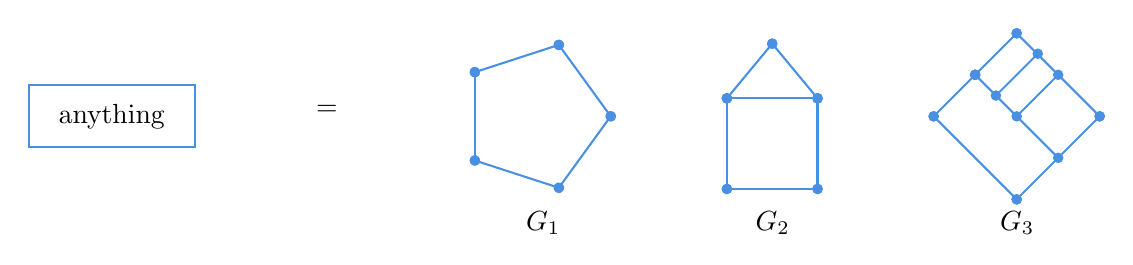
\begin{tikzpicture}[x=0.75pt,y=0.75pt,yscale=-1,xscale=1]
%uncomment if require: \path (0,107); %set diagram left start at 0, and has height of 107

%Shape: Rectangle [id:dp7714656589196636] 
\draw  [color={rgb, 255:red, 74; green, 144; blue, 226 }  ,draw opacity=1 ] (72,27.92) -- (152,27.92) -- (152,57.92) -- (72,57.92) -- cycle ;

%Straight Lines [id:da6038607286275557] 
\draw [color={rgb, 255:red, 74; green, 144; blue, 226 }  ,draw opacity=1 ]   (408.38,77.92) -- (408.38,34.26) ;
\draw [shift={(408.38,34.26)}, rotate = 270] [color={rgb, 255:red, 74; green, 144; blue, 226 }  ,draw opacity=1 ][fill={rgb, 255:red, 74; green, 144; blue, 226 }  ,fill opacity=1 ][line width=0.75]      (0, 0) circle [x radius= 2.01, y radius= 2.01]   ;
\draw [shift={(408.38,77.92)}, rotate = 270] [color={rgb, 255:red, 74; green, 144; blue, 226 }  ,draw opacity=1 ][fill={rgb, 255:red, 74; green, 144; blue, 226 }  ,fill opacity=1 ][line width=0.75]      (0, 0) circle [x radius= 2.01, y radius= 2.01]   ;
%Straight Lines [id:da6729271729627768] 
\draw [color={rgb, 255:red, 74; green, 144; blue, 226 }  ,draw opacity=1 ]   (408.38,77.92) -- (452.05,77.92) ;
\draw [shift={(452.05,77.92)}, rotate = 0] [color={rgb, 255:red, 74; green, 144; blue, 226 }  ,draw opacity=1 ][fill={rgb, 255:red, 74; green, 144; blue, 226 }  ,fill opacity=1 ][line width=0.75]      (0, 0) circle [x radius= 2.01, y radius= 2.01]   ;
\draw [shift={(408.38,77.92)}, rotate = 0] [color={rgb, 255:red, 74; green, 144; blue, 226 }  ,draw opacity=1 ][fill={rgb, 255:red, 74; green, 144; blue, 226 }  ,fill opacity=1 ][line width=0.75]      (0, 0) circle [x radius= 2.01, y radius= 2.01]   ;
%Straight Lines [id:da21534741015682468] 
\draw [color={rgb, 255:red, 74; green, 144; blue, 226 }  ,draw opacity=1 ]   (452.05,77.92) -- (452.05,34.26) ;
\draw [shift={(452.05,34.26)}, rotate = 270] [color={rgb, 255:red, 74; green, 144; blue, 226 }  ,draw opacity=1 ][fill={rgb, 255:red, 74; green, 144; blue, 226 }  ,fill opacity=1 ][line width=0.75]      (0, 0) circle [x radius= 2.01, y radius= 2.01]   ;
\draw [shift={(452.05,77.92)}, rotate = 270] [color={rgb, 255:red, 74; green, 144; blue, 226 }  ,draw opacity=1 ][fill={rgb, 255:red, 74; green, 144; blue, 226 }  ,fill opacity=1 ][line width=0.75]      (0, 0) circle [x radius= 2.01, y radius= 2.01]   ;
%Straight Lines [id:da9172996812005594] 
\draw [color={rgb, 255:red, 74; green, 144; blue, 226 }  ,draw opacity=1 ]   (430.22,7.92) -- (452.05,34.26) ;
\draw [shift={(452.05,34.26)}, rotate = 50.34] [color={rgb, 255:red, 74; green, 144; blue, 226 }  ,draw opacity=1 ][fill={rgb, 255:red, 74; green, 144; blue, 226 }  ,fill opacity=1 ][line width=0.75]      (0, 0) circle [x radius= 2.01, y radius= 2.01]   ;
\draw [shift={(430.22,7.92)}, rotate = 50.34] [color={rgb, 255:red, 74; green, 144; blue, 226 }  ,draw opacity=1 ][fill={rgb, 255:red, 74; green, 144; blue, 226 }  ,fill opacity=1 ][line width=0.75]      (0, 0) circle [x radius= 2.01, y radius= 2.01]   ;
%Straight Lines [id:da306566903160963] 
\draw [color={rgb, 255:red, 74; green, 144; blue, 226 }  ,draw opacity=1 ]   (408.38,34.26) -- (452.05,34.26) ;
\draw [shift={(452.05,34.26)}, rotate = 0] [color={rgb, 255:red, 74; green, 144; blue, 226 }  ,draw opacity=1 ][fill={rgb, 255:red, 74; green, 144; blue, 226 }  ,fill opacity=1 ][line width=0.75]      (0, 0) circle [x radius= 2.01, y radius= 2.01]   ;
\draw [shift={(408.38,34.26)}, rotate = 0] [color={rgb, 255:red, 74; green, 144; blue, 226 }  ,draw opacity=1 ][fill={rgb, 255:red, 74; green, 144; blue, 226 }  ,fill opacity=1 ][line width=0.75]      (0, 0) circle [x radius= 2.01, y radius= 2.01]   ;
%Straight Lines [id:da7150977941927978] 
\draw [color={rgb, 255:red, 74; green, 144; blue, 226 }  ,draw opacity=1 ]   (430.22,7.92) -- (408.38,34.26) ;
\draw [shift={(408.38,34.26)}, rotate = 129.66] [color={rgb, 255:red, 74; green, 144; blue, 226 }  ,draw opacity=1 ][fill={rgb, 255:red, 74; green, 144; blue, 226 }  ,fill opacity=1 ][line width=0.75]      (0, 0) circle [x radius= 2.01, y radius= 2.01]   ;
\draw [shift={(430.22,7.92)}, rotate = 129.66] [color={rgb, 255:red, 74; green, 144; blue, 226 }  ,draw opacity=1 ][fill={rgb, 255:red, 74; green, 144; blue, 226 }  ,fill opacity=1 ][line width=0.75]      (0, 0) circle [x radius= 2.01, y radius= 2.01]   ;

%Straight Lines [id:da49000811004443] 
\draw [color={rgb, 255:red, 74; green, 144; blue, 226 }  ,draw opacity=1 ]   (508,42.92) -- (548,82.92) ;
\draw [shift={(548,82.92)}, rotate = 45] [color={rgb, 255:red, 74; green, 144; blue, 226 }  ,draw opacity=1 ][fill={rgb, 255:red, 74; green, 144; blue, 226 }  ,fill opacity=1 ][line width=0.75]      (0, 0) circle [x radius= 2.01, y radius= 2.01]   ;
\draw [shift={(508,42.92)}, rotate = 45] [color={rgb, 255:red, 74; green, 144; blue, 226 }  ,draw opacity=1 ][fill={rgb, 255:red, 74; green, 144; blue, 226 }  ,fill opacity=1 ][line width=0.75]      (0, 0) circle [x radius= 2.01, y radius= 2.01]   ;
%Straight Lines [id:da002451494927559583] 
\draw [color={rgb, 255:red, 74; green, 144; blue, 226 }  ,draw opacity=1 ]   (568,22.92) -- (548,42.92) ;
\draw [shift={(548,42.92)}, rotate = 135] [color={rgb, 255:red, 74; green, 144; blue, 226 }  ,draw opacity=1 ][fill={rgb, 255:red, 74; green, 144; blue, 226 }  ,fill opacity=1 ][line width=0.75]      (0, 0) circle [x radius= 2.01, y radius= 2.01]   ;
\draw [shift={(568,22.92)}, rotate = 135] [color={rgb, 255:red, 74; green, 144; blue, 226 }  ,draw opacity=1 ][fill={rgb, 255:red, 74; green, 144; blue, 226 }  ,fill opacity=1 ][line width=0.75]      (0, 0) circle [x radius= 2.01, y radius= 2.01]   ;
%Straight Lines [id:da14744606135606264] 
\draw [color={rgb, 255:red, 74; green, 144; blue, 226 }  ,draw opacity=1 ]   (588,42.92) -- (548,82.92) ;
\draw [shift={(548,82.92)}, rotate = 135] [color={rgb, 255:red, 74; green, 144; blue, 226 }  ,draw opacity=1 ][fill={rgb, 255:red, 74; green, 144; blue, 226 }  ,fill opacity=1 ][line width=0.75]      (0, 0) circle [x radius= 2.01, y radius= 2.01]   ;
\draw [shift={(588,42.92)}, rotate = 135] [color={rgb, 255:red, 74; green, 144; blue, 226 }  ,draw opacity=1 ][fill={rgb, 255:red, 74; green, 144; blue, 226 }  ,fill opacity=1 ][line width=0.75]      (0, 0) circle [x radius= 2.01, y radius= 2.01]   ;
%Straight Lines [id:da8494141085185327] 
\draw [color={rgb, 255:red, 74; green, 144; blue, 226 }  ,draw opacity=1 ]   (528,22.92) -- (548,2.92) ;
\draw [shift={(548,2.92)}, rotate = 315] [color={rgb, 255:red, 74; green, 144; blue, 226 }  ,draw opacity=1 ][fill={rgb, 255:red, 74; green, 144; blue, 226 }  ,fill opacity=1 ][line width=0.75]      (0, 0) circle [x radius= 2.01, y radius= 2.01]   ;
\draw [shift={(528,22.92)}, rotate = 315] [color={rgb, 255:red, 74; green, 144; blue, 226 }  ,draw opacity=1 ][fill={rgb, 255:red, 74; green, 144; blue, 226 }  ,fill opacity=1 ][line width=0.75]      (0, 0) circle [x radius= 2.01, y radius= 2.01]   ;
%Straight Lines [id:da6243812307279271] 
\draw [color={rgb, 255:red, 74; green, 144; blue, 226 }  ,draw opacity=1 ]   (508,42.92) -- (528,22.92) ;
\draw [shift={(528,22.92)}, rotate = 315] [color={rgb, 255:red, 74; green, 144; blue, 226 }  ,draw opacity=1 ][fill={rgb, 255:red, 74; green, 144; blue, 226 }  ,fill opacity=1 ][line width=0.75]      (0, 0) circle [x radius= 2.01, y radius= 2.01]   ;
\draw [shift={(508,42.92)}, rotate = 315] [color={rgb, 255:red, 74; green, 144; blue, 226 }  ,draw opacity=1 ][fill={rgb, 255:red, 74; green, 144; blue, 226 }  ,fill opacity=1 ][line width=0.75]      (0, 0) circle [x radius= 2.01, y radius= 2.01]   ;
%Straight Lines [id:da5121179547828358] 
\draw [color={rgb, 255:red, 74; green, 144; blue, 226 }  ,draw opacity=1 ]   (568,62.92) -- (528,22.92) ;
\draw [shift={(528,22.92)}, rotate = 225] [color={rgb, 255:red, 74; green, 144; blue, 226 }  ,draw opacity=1 ][fill={rgb, 255:red, 74; green, 144; blue, 226 }  ,fill opacity=1 ][line width=0.75]      (0, 0) circle [x radius= 2.01, y radius= 2.01]   ;
\draw [shift={(568,62.92)}, rotate = 225] [color={rgb, 255:red, 74; green, 144; blue, 226 }  ,draw opacity=1 ][fill={rgb, 255:red, 74; green, 144; blue, 226 }  ,fill opacity=1 ][line width=0.75]      (0, 0) circle [x radius= 2.01, y radius= 2.01]   ;
%Straight Lines [id:da030965817685151498] 
\draw [color={rgb, 255:red, 74; green, 144; blue, 226 }  ,draw opacity=1 ]   (588,42.92) -- (548,2.92) ;
\draw [shift={(548,2.92)}, rotate = 225] [color={rgb, 255:red, 74; green, 144; blue, 226 }  ,draw opacity=1 ][fill={rgb, 255:red, 74; green, 144; blue, 226 }  ,fill opacity=1 ][line width=0.75]      (0, 0) circle [x radius= 2.01, y radius= 2.01]   ;
\draw [shift={(588,42.92)}, rotate = 225] [color={rgb, 255:red, 74; green, 144; blue, 226 }  ,draw opacity=1 ][fill={rgb, 255:red, 74; green, 144; blue, 226 }  ,fill opacity=1 ][line width=0.75]      (0, 0) circle [x radius= 2.01, y radius= 2.01]   ;
%Straight Lines [id:da9487634255003965] 
\draw [color={rgb, 255:red, 74; green, 144; blue, 226 }  ,draw opacity=1 ]   (538,32.92) -- (558.16,12.77) ;
\draw [shift={(558.16,12.77)}, rotate = 315] [color={rgb, 255:red, 74; green, 144; blue, 226 }  ,draw opacity=1 ][fill={rgb, 255:red, 74; green, 144; blue, 226 }  ,fill opacity=1 ][line width=0.75]      (0, 0) circle [x radius= 2.01, y radius= 2.01]   ;
\draw [shift={(538,32.92)}, rotate = 315] [color={rgb, 255:red, 74; green, 144; blue, 226 }  ,draw opacity=1 ][fill={rgb, 255:red, 74; green, 144; blue, 226 }  ,fill opacity=1 ][line width=0.75]      (0, 0) circle [x radius= 2.01, y radius= 2.01]   ;

%Straight Lines [id:da8492214114013805] 
\draw [color={rgb, 255:red, 74; green, 144; blue, 226 }  ,draw opacity=1 ]   (327.4,77.34) -- (352.41,42.92) ;
\draw [shift={(352.41,42.92)}, rotate = 306] [color={rgb, 255:red, 74; green, 144; blue, 226 }  ,draw opacity=1 ][fill={rgb, 255:red, 74; green, 144; blue, 226 }  ,fill opacity=1 ][line width=0.75]      (0, 0) circle [x radius= 2.01, y radius= 2.01]   ;
\draw [shift={(327.4,77.34)}, rotate = 306] [color={rgb, 255:red, 74; green, 144; blue, 226 }  ,draw opacity=1 ][fill={rgb, 255:red, 74; green, 144; blue, 226 }  ,fill opacity=1 ][line width=0.75]      (0, 0) circle [x radius= 2.01, y radius= 2.01]   ;
%Straight Lines [id:da8163370212559675] 
\draw [color={rgb, 255:red, 74; green, 144; blue, 226 }  ,draw opacity=1 ]   (327.4,77.34) -- (286.94,64.2) ;
\draw [shift={(286.94,64.2)}, rotate = 198] [color={rgb, 255:red, 74; green, 144; blue, 226 }  ,draw opacity=1 ][fill={rgb, 255:red, 74; green, 144; blue, 226 }  ,fill opacity=1 ][line width=0.75]      (0, 0) circle [x radius= 2.01, y radius= 2.01]   ;
\draw [shift={(327.4,77.34)}, rotate = 198] [color={rgb, 255:red, 74; green, 144; blue, 226 }  ,draw opacity=1 ][fill={rgb, 255:red, 74; green, 144; blue, 226 }  ,fill opacity=1 ][line width=0.75]      (0, 0) circle [x radius= 2.01, y radius= 2.01]   ;
%Straight Lines [id:da8052406048989194] 
\draw [color={rgb, 255:red, 74; green, 144; blue, 226 }  ,draw opacity=1 ]   (352.41,42.92) -- (327.4,8.5) ;
\draw [shift={(327.4,8.5)}, rotate = 234] [color={rgb, 255:red, 74; green, 144; blue, 226 }  ,draw opacity=1 ][fill={rgb, 255:red, 74; green, 144; blue, 226 }  ,fill opacity=1 ][line width=0.75]      (0, 0) circle [x radius= 2.01, y radius= 2.01]   ;
\draw [shift={(352.41,42.92)}, rotate = 234] [color={rgb, 255:red, 74; green, 144; blue, 226 }  ,draw opacity=1 ][fill={rgb, 255:red, 74; green, 144; blue, 226 }  ,fill opacity=1 ][line width=0.75]      (0, 0) circle [x radius= 2.01, y radius= 2.01]   ;
%Straight Lines [id:da6891281226234369] 
\draw [color={rgb, 255:red, 74; green, 144; blue, 226 }  ,draw opacity=1 ]   (286.94,21.65) -- (327.4,8.5) ;
\draw [shift={(327.4,8.5)}, rotate = 342] [color={rgb, 255:red, 74; green, 144; blue, 226 }  ,draw opacity=1 ][fill={rgb, 255:red, 74; green, 144; blue, 226 }  ,fill opacity=1 ][line width=0.75]      (0, 0) circle [x radius= 2.01, y radius= 2.01]   ;
\draw [shift={(286.94,21.65)}, rotate = 342] [color={rgb, 255:red, 74; green, 144; blue, 226 }  ,draw opacity=1 ][fill={rgb, 255:red, 74; green, 144; blue, 226 }  ,fill opacity=1 ][line width=0.75]      (0, 0) circle [x radius= 2.01, y radius= 2.01]   ;
%Straight Lines [id:da8647450658189417] 
\draw [color={rgb, 255:red, 74; green, 144; blue, 226 }  ,draw opacity=1 ]   (286.94,64.2) -- (286.94,21.65) ;
\draw [shift={(286.94,21.65)}, rotate = 270] [color={rgb, 255:red, 74; green, 144; blue, 226 }  ,draw opacity=1 ][fill={rgb, 255:red, 74; green, 144; blue, 226 }  ,fill opacity=1 ][line width=0.75]      (0, 0) circle [x radius= 2.01, y radius= 2.01]   ;
\draw [shift={(286.94,64.2)}, rotate = 270] [color={rgb, 255:red, 74; green, 144; blue, 226 }  ,draw opacity=1 ][fill={rgb, 255:red, 74; green, 144; blue, 226 }  ,fill opacity=1 ][line width=0.75]      (0, 0) circle [x radius= 2.01, y radius= 2.01]   ;


% Text Node
\draw (208.97,35.92) node [anchor=north west][inner sep=0.75pt]    {$=$};
% Text Node
\draw (112,42.92) node   [align=left] {anything};
% Text Node
\draw (310.18,87.49) node [anchor=north west][inner sep=0.75pt]    {$G_{1}$};
% Text Node
\draw (420.72,87.49) node [anchor=north west][inner sep=0.75pt]    {$G_{2}$};
% Text Node
\draw (538.5,87.49) node [anchor=north west][inner sep=0.75pt]    {$G_{3}$};
\end{tikzpicture}
\caption{Three examples of the algorithm.}
\label{fig:G1G2G3}
\end{figure}

For graph $G_{1}$:
\begin{equation*}
\tikzset{every picture/.style={line width=0.75pt}} %set default line width to 0.75pt        
\begin{tikzpicture}[x=0.75pt,y=0.75pt,yscale=-1,xscale=1, baseline=(XXXX.south) ]
\path (0,139);\path (80.99545288085938,0);\draw    ($(current bounding box.center)+(0,0.3em)$) node [anchor=south] (XXXX) {};
%Straight Lines [id:da05619945871347576] 
\draw [color={rgb, 255:red, 74; green, 144; blue, 226 }  ,draw opacity=1 ]   (51.5,100.34) -- (76.5,65.92) ;
\draw [shift={(76.5,65.92)}, rotate = 306] [color={rgb, 255:red, 74; green, 144; blue, 226 }  ,draw opacity=1 ][fill={rgb, 255:red, 74; green, 144; blue, 226 }  ,fill opacity=1 ][line width=0.75]      (0, 0) circle [x radius= 2.01, y radius= 2.01]   ;
\draw [shift={(51.5,100.34)}, rotate = 306] [color={rgb, 255:red, 74; green, 144; blue, 226 }  ,draw opacity=1 ][fill={rgb, 255:red, 74; green, 144; blue, 226 }  ,fill opacity=1 ][line width=0.75]      (0, 0) circle [x radius= 2.01, y radius= 2.01]   ;
%Straight Lines [id:da6223307112307022] 
\draw [color={rgb, 255:red, 74; green, 144; blue, 226 }  ,draw opacity=1 ]   (51.5,100.34) -- (11.03,87.2) ;
\draw [shift={(11.03,87.2)}, rotate = 198] [color={rgb, 255:red, 74; green, 144; blue, 226 }  ,draw opacity=1 ][fill={rgb, 255:red, 74; green, 144; blue, 226 }  ,fill opacity=1 ][line width=0.75]      (0, 0) circle [x radius= 2.01, y radius= 2.01]   ;
\draw [shift={(51.5,100.34)}, rotate = 198] [color={rgb, 255:red, 74; green, 144; blue, 226 }  ,draw opacity=1 ][fill={rgb, 255:red, 74; green, 144; blue, 226 }  ,fill opacity=1 ][line width=0.75]      (0, 0) circle [x radius= 2.01, y radius= 2.01]   ;
%Straight Lines [id:da37090835708948733] 
\draw [color={rgb, 255:red, 74; green, 144; blue, 226 }  ,draw opacity=1 ]   (76.5,65.92) -- (51.5,31.5) ;
\draw [shift={(51.5,31.5)}, rotate = 234] [color={rgb, 255:red, 74; green, 144; blue, 226 }  ,draw opacity=1 ][fill={rgb, 255:red, 74; green, 144; blue, 226 }  ,fill opacity=1 ][line width=0.75]      (0, 0) circle [x radius= 2.01, y radius= 2.01]   ;
\draw [shift={(76.5,65.92)}, rotate = 234] [color={rgb, 255:red, 74; green, 144; blue, 226 }  ,draw opacity=1 ][fill={rgb, 255:red, 74; green, 144; blue, 226 }  ,fill opacity=1 ][line width=0.75]      (0, 0) circle [x radius= 2.01, y radius= 2.01]   ;
%Straight Lines [id:da04657766702833066] 
\draw [color={rgb, 255:red, 74; green, 144; blue, 226 }  ,draw opacity=1 ]   (11.03,44.65) -- (51.5,31.5) ;
\draw [shift={(51.5,31.5)}, rotate = 342] [color={rgb, 255:red, 74; green, 144; blue, 226 }  ,draw opacity=1 ][fill={rgb, 255:red, 74; green, 144; blue, 226 }  ,fill opacity=1 ][line width=0.75]      (0, 0) circle [x radius= 2.01, y radius= 2.01]   ;
\draw [shift={(11.03,44.65)}, rotate = 342] [color={rgb, 255:red, 74; green, 144; blue, 226 }  ,draw opacity=1 ][fill={rgb, 255:red, 74; green, 144; blue, 226 }  ,fill opacity=1 ][line width=0.75]      (0, 0) circle [x radius= 2.01, y radius= 2.01]   ;
%Straight Lines [id:da15681820978770467] 
\draw [color={rgb, 255:red, 74; green, 144; blue, 226 }  ,draw opacity=1 ]   (11.03,87.2) -- (11.03,44.65) ;
\draw [shift={(11.03,44.65)}, rotate = 270] [color={rgb, 255:red, 74; green, 144; blue, 226 }  ,draw opacity=1 ][fill={rgb, 255:red, 74; green, 144; blue, 226 }  ,fill opacity=1 ][line width=0.75]      (0, 0) circle [x radius= 2.01, y radius= 2.01]   ;
\draw [shift={(11.03,87.2)}, rotate = 270] [color={rgb, 255:red, 74; green, 144; blue, 226 }  ,draw opacity=1 ][fill={rgb, 255:red, 74; green, 144; blue, 226 }  ,fill opacity=1 ][line width=0.75]      (0, 0) circle [x radius= 2.01, y radius= 2.01]   ;
%Straight Lines [id:da563569033314038] 
\draw [color={rgb, 255:red, 74; green, 144; blue, 226 }  ,draw opacity=1 ]   (51.5,133.88) -- (51.5,100.34) ;
\draw [shift={(51.5,100.34)}, rotate = 270] [color={rgb, 255:red, 74; green, 144; blue, 226 }  ,draw opacity=1 ][fill={rgb, 255:red, 74; green, 144; blue, 226 }  ,fill opacity=1 ][line width=0.75]      (0, 0) circle [x radius= 2.01, y radius= 2.01]   ;
\draw [shift={(51.5,133.88)}, rotate = 270] [color={rgb, 255:red, 74; green, 144; blue, 226 }  ,draw opacity=1 ][fill={rgb, 255:red, 74; green, 144; blue, 226 }  ,fill opacity=1 ][line width=0.75]      (0, 0) circle [x radius= 2.01, y radius= 2.01]   ;
%Straight Lines [id:da3682767032370169] 
\draw [color={rgb, 255:red, 74; green, 144; blue, 226 }  ,draw opacity=1 ]   (51.5,31.5) -- (51.5,2.97) ;
\draw [shift={(51.5,2.97)}, rotate = 270] [color={rgb, 255:red, 74; green, 144; blue, 226 }  ,draw opacity=1 ][fill={rgb, 255:red, 74; green, 144; blue, 226 }  ,fill opacity=1 ][line width=0.75]      (0, 0) circle [x radius= 2.01, y radius= 2.01]   ;
\draw [shift={(51.5,31.5)}, rotate = 270] [color={rgb, 255:red, 74; green, 144; blue, 226 }  ,draw opacity=1 ][fill={rgb, 255:red, 74; green, 144; blue, 226 }  ,fill opacity=1 ][line width=0.75]      (0, 0) circle [x radius= 2.01, y radius= 2.01]   ;
% Text Node
\draw (33.09,110.5) node [anchor=north west][inner sep=0.75pt]    {$a$};
% Text Node
\draw (33.09,8.5) node [anchor=north west][inner sep=0.75pt]    {$b$};
% Text Node
\draw (23.09,92.5) node [anchor=north west][inner sep=0.75pt]    {$c$};
% Text Node
\draw (67,78.63) node [anchor=north west][inner sep=0.75pt]    {$d$};
% Text Node
\draw (-1.91,56.5) node [anchor=north west][inner sep=0.75pt]    {$e$};
% Text Node
\draw (18.26,20.58) node [anchor=north west][inner sep=0.75pt]    {$f$};
% Text Node
\draw (66.09,32.5) node [anchor=north west][inner sep=0.75pt]    {$g$};
\end{tikzpicture}
=\delta _{ec}\tikzset{every picture/.style={line width=0.75pt}} %set default line width to 0.75pt        
\begin{tikzpicture}[x=0.75pt,y=0.75pt,yscale=-1,xscale=1, baseline=(XXXX.south) ]
\path (0,139);\path (62.99273681640625,0);\draw    ($(current bounding box.center)+(0,0.3em)$) node [anchor=south] (XXXX) {};
%Straight Lines [id:da7599761611877247] 
\draw [color={rgb, 255:red, 74; green, 144; blue, 226 }  ,draw opacity=1 ]   (30.49,102.33) -- (55.5,67.91) ;
\draw [shift={(55.5,67.91)}, rotate = 306] [color={rgb, 255:red, 74; green, 144; blue, 226 }  ,draw opacity=1 ][fill={rgb, 255:red, 74; green, 144; blue, 226 }  ,fill opacity=1 ][line width=0.75]      (0, 0) circle [x radius= 2.01, y radius= 2.01]   ;
\draw [shift={(30.49,102.33)}, rotate = 306] [color={rgb, 255:red, 74; green, 144; blue, 226 }  ,draw opacity=1 ][fill={rgb, 255:red, 74; green, 144; blue, 226 }  ,fill opacity=1 ][line width=0.75]      (0, 0) circle [x radius= 2.01, y radius= 2.01]   ;
%Straight Lines [id:da48220189914045086] 
\draw [color={rgb, 255:red, 74; green, 144; blue, 226 }  ,draw opacity=1 ]   (55.5,67.91) -- (30.49,33.49) ;
\draw [shift={(30.49,33.49)}, rotate = 234] [color={rgb, 255:red, 74; green, 144; blue, 226 }  ,draw opacity=1 ][fill={rgb, 255:red, 74; green, 144; blue, 226 }  ,fill opacity=1 ][line width=0.75]      (0, 0) circle [x radius= 2.01, y radius= 2.01]   ;
\draw [shift={(55.5,67.91)}, rotate = 234] [color={rgb, 255:red, 74; green, 144; blue, 226 }  ,draw opacity=1 ][fill={rgb, 255:red, 74; green, 144; blue, 226 }  ,fill opacity=1 ][line width=0.75]      (0, 0) circle [x radius= 2.01, y radius= 2.01]   ;
%Straight Lines [id:da6918702166920927] 
\draw [color={rgb, 255:red, 74; green, 144; blue, 226 }  ,draw opacity=1 ]   (30.49,135.87) -- (30.49,102.33) ;
\draw [shift={(30.49,102.33)}, rotate = 270] [color={rgb, 255:red, 74; green, 144; blue, 226 }  ,draw opacity=1 ][fill={rgb, 255:red, 74; green, 144; blue, 226 }  ,fill opacity=1 ][line width=0.75]      (0, 0) circle [x radius= 2.01, y radius= 2.01]   ;
\draw [shift={(30.49,135.87)}, rotate = 270] [color={rgb, 255:red, 74; green, 144; blue, 226 }  ,draw opacity=1 ][fill={rgb, 255:red, 74; green, 144; blue, 226 }  ,fill opacity=1 ][line width=0.75]      (0, 0) circle [x radius= 2.01, y radius= 2.01]   ;
%Straight Lines [id:da6071842094533277] 
\draw [color={rgb, 255:red, 74; green, 144; blue, 226 }  ,draw opacity=1 ]   (30.49,33.49) -- (30.49,4.95) ;
\draw [shift={(30.49,4.95)}, rotate = 270] [color={rgb, 255:red, 74; green, 144; blue, 226 }  ,draw opacity=1 ][fill={rgb, 255:red, 74; green, 144; blue, 226 }  ,fill opacity=1 ][line width=0.75]      (0, 0) circle [x radius= 2.01, y radius= 2.01]   ;
\draw [shift={(30.49,33.49)}, rotate = 270] [color={rgb, 255:red, 74; green, 144; blue, 226 }  ,draw opacity=1 ][fill={rgb, 255:red, 74; green, 144; blue, 226 }  ,fill opacity=1 ][line width=0.75]      (0, 0) circle [x radius= 2.01, y radius= 2.01]   ;
%Straight Lines [id:da9059245541527421] 
\draw [color={rgb, 255:red, 74; green, 144; blue, 226 }  ,draw opacity=1 ]   (30.49,102.33) -- (5.48,67.91) ;
\draw [shift={(5.48,67.91)}, rotate = 234] [color={rgb, 255:red, 74; green, 144; blue, 226 }  ,draw opacity=1 ][fill={rgb, 255:red, 74; green, 144; blue, 226 }  ,fill opacity=1 ][line width=0.75]      (0, 0) circle [x radius= 2.01, y radius= 2.01]   ;
\draw [shift={(30.49,102.33)}, rotate = 234] [color={rgb, 255:red, 74; green, 144; blue, 226 }  ,draw opacity=1 ][fill={rgb, 255:red, 74; green, 144; blue, 226 }  ,fill opacity=1 ][line width=0.75]      (0, 0) circle [x radius= 2.01, y radius= 2.01]   ;
%Straight Lines [id:da491715002930452] 
\draw [color={rgb, 255:red, 74; green, 144; blue, 226 }  ,draw opacity=1 ]   (5.48,67.91) -- (30.49,33.49) ;
\draw [shift={(30.49,33.49)}, rotate = 306] [color={rgb, 255:red, 74; green, 144; blue, 226 }  ,draw opacity=1 ][fill={rgb, 255:red, 74; green, 144; blue, 226 }  ,fill opacity=1 ][line width=0.75]      (0, 0) circle [x radius= 2.01, y radius= 2.01]   ;
\draw [shift={(5.48,67.91)}, rotate = 306] [color={rgb, 255:red, 74; green, 144; blue, 226 }  ,draw opacity=1 ][fill={rgb, 255:red, 74; green, 144; blue, 226 }  ,fill opacity=1 ][line width=0.75]      (0, 0) circle [x radius= 2.01, y radius= 2.01]   ;
% Text Node
\draw (12.09,112.49) node [anchor=north west][inner sep=0.75pt]    {$a$};
% Text Node
\draw (12.09,10.49) node [anchor=north west][inner sep=0.75pt]    {$b$};
% Text Node
\draw (3.09,83.49) node [anchor=north west][inner sep=0.75pt]    {$c$};
% Text Node
\draw (48,83.62) node [anchor=north west][inner sep=0.75pt]    {$d$};
% Text Node
\draw (6.26,37.56) node [anchor=north west][inner sep=0.75pt]    {$f$};
% Text Node
\draw (47.09,37.49) node [anchor=north west][inner sep=0.75pt]    {$g$};
\end{tikzpicture}
=\delta _{ec} \delta _{cf} \delta _{gd} \delta _{ab}\tikzset{every picture/.style={line width=0.75pt}} %set default line width to 0.75pt        
\begin{tikzpicture}[x=0.75pt,y=0.75pt,yscale=-1,xscale=1, baseline=(XXXX.south) ]
\path (0,108);\path (18.991836547851562,0);\draw    ($(current bounding box.center)+(0,0.3em)$) node [anchor=south] (XXXX) {};
%Straight Lines [id:da4609445021441321] 
\draw [color={rgb, 255:red, 74; green, 144; blue, 226 }  ,draw opacity=1 ]   (4,4) -- (4,105.51) ;
% Text Node
\draw (8,47.5) node [anchor=north west][inner sep=0.75pt]    {$a$};
\end{tikzpicture}
.
\end{equation*}
For graph $G_{2}$:
\begin{equation*}
\tikzset{every picture/.style={line width=0.75pt}} %set default line width to 0.75pt        
\begin{tikzpicture}[x=0.75pt,y=0.75pt,yscale=-1,xscale=1, baseline=(XXXX.south) ]
\path (0,112);\path (89.99652099609375,0);\draw    ($(current bounding box.center)+(0,0.3em)$) node [anchor=south] (XXXX) {};
%Straight Lines [id:da930464172631351] 
\draw [color={rgb, 255:red, 74; green, 144; blue, 226 }  ,draw opacity=1 ]   (72.72,75.75) -- (29.05,75.75) ;
\draw [shift={(29.05,75.75)}, rotate = 180] [color={rgb, 255:red, 74; green, 144; blue, 226 }  ,draw opacity=1 ][fill={rgb, 255:red, 74; green, 144; blue, 226 }  ,fill opacity=1 ][line width=0.75]      (0, 0) circle [x radius= 2.01, y radius= 2.01]   ;
\draw [shift={(72.72,75.75)}, rotate = 180] [color={rgb, 255:red, 74; green, 144; blue, 226 }  ,draw opacity=1 ][fill={rgb, 255:red, 74; green, 144; blue, 226 }  ,fill opacity=1 ][line width=0.75]      (0, 0) circle [x radius= 2.01, y radius= 2.01]   ;
%Straight Lines [id:da8547208824043067] 
\draw [color={rgb, 255:red, 74; green, 144; blue, 226 }  ,draw opacity=1 ]   (72.72,75.75) -- (72.72,32.09) ;
\draw [shift={(72.72,32.09)}, rotate = 270] [color={rgb, 255:red, 74; green, 144; blue, 226 }  ,draw opacity=1 ][fill={rgb, 255:red, 74; green, 144; blue, 226 }  ,fill opacity=1 ][line width=0.75]      (0, 0) circle [x radius= 2.01, y radius= 2.01]   ;
\draw [shift={(72.72,75.75)}, rotate = 270] [color={rgb, 255:red, 74; green, 144; blue, 226 }  ,draw opacity=1 ][fill={rgb, 255:red, 74; green, 144; blue, 226 }  ,fill opacity=1 ][line width=0.75]      (0, 0) circle [x radius= 2.01, y radius= 2.01]   ;
%Straight Lines [id:da4429024782112838] 
\draw [color={rgb, 255:red, 74; green, 144; blue, 226 }  ,draw opacity=1 ]   (72.72,32.09) -- (29.05,32.09) ;
\draw [shift={(29.05,32.09)}, rotate = 180] [color={rgb, 255:red, 74; green, 144; blue, 226 }  ,draw opacity=1 ][fill={rgb, 255:red, 74; green, 144; blue, 226 }  ,fill opacity=1 ][line width=0.75]      (0, 0) circle [x radius= 2.01, y radius= 2.01]   ;
\draw [shift={(72.72,32.09)}, rotate = 180] [color={rgb, 255:red, 74; green, 144; blue, 226 }  ,draw opacity=1 ][fill={rgb, 255:red, 74; green, 144; blue, 226 }  ,fill opacity=1 ][line width=0.75]      (0, 0) circle [x radius= 2.01, y radius= 2.01]   ;
%Straight Lines [id:da8297072051993224] 
\draw [color={rgb, 255:red, 74; green, 144; blue, 226 }  ,draw opacity=1 ]   (2.72,53.92) -- (29.05,32.09) ;
\draw [shift={(29.05,32.09)}, rotate = 320.34] [color={rgb, 255:red, 74; green, 144; blue, 226 }  ,draw opacity=1 ][fill={rgb, 255:red, 74; green, 144; blue, 226 }  ,fill opacity=1 ][line width=0.75]      (0, 0) circle [x radius= 2.01, y radius= 2.01]   ;
\draw [shift={(2.72,53.92)}, rotate = 320.34] [color={rgb, 255:red, 74; green, 144; blue, 226 }  ,draw opacity=1 ][fill={rgb, 255:red, 74; green, 144; blue, 226 }  ,fill opacity=1 ][line width=0.75]      (0, 0) circle [x radius= 2.01, y radius= 2.01]   ;
%Straight Lines [id:da18250197718884786] 
\draw [color={rgb, 255:red, 74; green, 144; blue, 226 }  ,draw opacity=1 ]   (29.05,75.75) -- (29.05,32.09) ;
\draw [shift={(29.05,32.09)}, rotate = 270] [color={rgb, 255:red, 74; green, 144; blue, 226 }  ,draw opacity=1 ][fill={rgb, 255:red, 74; green, 144; blue, 226 }  ,fill opacity=1 ][line width=0.75]      (0, 0) circle [x radius= 2.01, y radius= 2.01]   ;
\draw [shift={(29.05,75.75)}, rotate = 270] [color={rgb, 255:red, 74; green, 144; blue, 226 }  ,draw opacity=1 ][fill={rgb, 255:red, 74; green, 144; blue, 226 }  ,fill opacity=1 ][line width=0.75]      (0, 0) circle [x radius= 2.01, y radius= 2.01]   ;
%Straight Lines [id:da2722413239210222] 
\draw [color={rgb, 255:red, 74; green, 144; blue, 226 }  ,draw opacity=1 ]   (2.72,53.92) -- (29.05,75.75) ;
\draw [shift={(29.05,75.75)}, rotate = 39.66] [color={rgb, 255:red, 74; green, 144; blue, 226 }  ,draw opacity=1 ][fill={rgb, 255:red, 74; green, 144; blue, 226 }  ,fill opacity=1 ][line width=0.75]      (0, 0) circle [x radius= 2.01, y radius= 2.01]   ;
\draw [shift={(2.72,53.92)}, rotate = 39.66] [color={rgb, 255:red, 74; green, 144; blue, 226 }  ,draw opacity=1 ][fill={rgb, 255:red, 74; green, 144; blue, 226 }  ,fill opacity=1 ][line width=0.75]      (0, 0) circle [x radius= 2.01, y radius= 2.01]   ;
%Straight Lines [id:da7088038765322597] 
\draw [color={rgb, 255:red, 74; green, 144; blue, 226 }  ,draw opacity=1 ]   (72.72,109.29) -- (72.72,75.75) ;
\draw [shift={(72.72,75.75)}, rotate = 270] [color={rgb, 255:red, 74; green, 144; blue, 226 }  ,draw opacity=1 ][fill={rgb, 255:red, 74; green, 144; blue, 226 }  ,fill opacity=1 ][line width=0.75]      (0, 0) circle [x radius= 2.01, y radius= 2.01]   ;
\draw [shift={(72.72,109.29)}, rotate = 270] [color={rgb, 255:red, 74; green, 144; blue, 226 }  ,draw opacity=1 ][fill={rgb, 255:red, 74; green, 144; blue, 226 }  ,fill opacity=1 ][line width=0.75]      (0, 0) circle [x radius= 2.01, y radius= 2.01]   ;
%Straight Lines [id:da403678726206107] 
\draw [color={rgb, 255:red, 74; green, 144; blue, 226 }  ,draw opacity=1 ]   (72.72,32.09) -- (72.72,3.55) ;
\draw [shift={(72.72,3.55)}, rotate = 270] [color={rgb, 255:red, 74; green, 144; blue, 226 }  ,draw opacity=1 ][fill={rgb, 255:red, 74; green, 144; blue, 226 }  ,fill opacity=1 ][line width=0.75]      (0, 0) circle [x radius= 2.01, y radius= 2.01]   ;
\draw [shift={(72.72,32.09)}, rotate = 270] [color={rgb, 255:red, 74; green, 144; blue, 226 }  ,draw opacity=1 ][fill={rgb, 255:red, 74; green, 144; blue, 226 }  ,fill opacity=1 ][line width=0.75]      (0, 0) circle [x radius= 2.01, y radius= 2.01]   ;
% Text Node
\draw (80,83.5) node [anchor=north west][inner sep=0.75pt]    {$a$};
% Text Node
\draw (80,11.5) node [anchor=north west][inner sep=0.75pt]    {$b$};
% Text Node
\draw (80,45.5) node [anchor=north west][inner sep=0.75pt]    {$c$};
% Text Node
\draw (46.45,74.63) node [anchor=north west][inner sep=0.75pt]    {$d$};
% Text Node
\draw (7.59,61.5) node [anchor=north west][inner sep=0.75pt]    {$e$};
% Text Node
\draw (7.59,26.58) node [anchor=north west][inner sep=0.75pt]    {$f$};
% Text Node
\draw (31.5,43.5) node [anchor=north west][inner sep=0.75pt]    {$g$};
% Text Node
\draw (46.45,12.5) node [anchor=north west][inner sep=0.75pt]    {$h$};
\end{tikzpicture}
=\delta _{ef}\tikzset{every picture/.style={line width=0.75pt}} %set default line width to 0.75pt        
\begin{tikzpicture}[x=0.75pt,y=0.75pt,yscale=-1,xscale=1, baseline=(XXXX.south) ]
\path (0,112);\path (99.99478912353516,0);\draw    ($(current bounding box.center)+(0,0.3em)$) node [anchor=south] (XXXX) {};
%Straight Lines [id:da7406870516171276] 
\draw [color={rgb, 255:red, 74; green, 144; blue, 226 }  ,draw opacity=1 ]   (78.71,74.75) -- (35.05,74.75) ;
\draw [shift={(35.05,74.75)}, rotate = 180] [color={rgb, 255:red, 74; green, 144; blue, 226 }  ,draw opacity=1 ][fill={rgb, 255:red, 74; green, 144; blue, 226 }  ,fill opacity=1 ][line width=0.75]      (0, 0) circle [x radius= 2.01, y radius= 2.01]   ;
\draw [shift={(78.71,74.75)}, rotate = 180] [color={rgb, 255:red, 74; green, 144; blue, 226 }  ,draw opacity=1 ][fill={rgb, 255:red, 74; green, 144; blue, 226 }  ,fill opacity=1 ][line width=0.75]      (0, 0) circle [x radius= 2.01, y radius= 2.01]   ;
%Straight Lines [id:da9911232645175818] 
\draw [color={rgb, 255:red, 74; green, 144; blue, 226 }  ,draw opacity=1 ]   (78.71,74.75) -- (78.71,31.08) ;
\draw [shift={(78.71,31.08)}, rotate = 270] [color={rgb, 255:red, 74; green, 144; blue, 226 }  ,draw opacity=1 ][fill={rgb, 255:red, 74; green, 144; blue, 226 }  ,fill opacity=1 ][line width=0.75]      (0, 0) circle [x radius= 2.01, y radius= 2.01]   ;
\draw [shift={(78.71,74.75)}, rotate = 270] [color={rgb, 255:red, 74; green, 144; blue, 226 }  ,draw opacity=1 ][fill={rgb, 255:red, 74; green, 144; blue, 226 }  ,fill opacity=1 ][line width=0.75]      (0, 0) circle [x radius= 2.01, y radius= 2.01]   ;
%Straight Lines [id:da22943156706569856] 
\draw [color={rgb, 255:red, 74; green, 144; blue, 226 }  ,draw opacity=1 ]   (78.71,31.08) -- (35.05,31.08) ;
\draw [shift={(35.05,31.08)}, rotate = 180] [color={rgb, 255:red, 74; green, 144; blue, 226 }  ,draw opacity=1 ][fill={rgb, 255:red, 74; green, 144; blue, 226 }  ,fill opacity=1 ][line width=0.75]      (0, 0) circle [x radius= 2.01, y radius= 2.01]   ;
\draw [shift={(78.71,31.08)}, rotate = 180] [color={rgb, 255:red, 74; green, 144; blue, 226 }  ,draw opacity=1 ][fill={rgb, 255:red, 74; green, 144; blue, 226 }  ,fill opacity=1 ][line width=0.75]      (0, 0) circle [x radius= 2.01, y radius= 2.01]   ;
%Straight Lines [id:da2315485460001665] 
\draw [color={rgb, 255:red, 74; green, 144; blue, 226 }  ,draw opacity=1 ]   (35.05,74.75) -- (35.05,31.08) ;
\draw [shift={(35.05,31.08)}, rotate = 270] [color={rgb, 255:red, 74; green, 144; blue, 226 }  ,draw opacity=1 ][fill={rgb, 255:red, 74; green, 144; blue, 226 }  ,fill opacity=1 ][line width=0.75]      (0, 0) circle [x radius= 2.01, y radius= 2.01]   ;
\draw [shift={(35.05,74.75)}, rotate = 270] [color={rgb, 255:red, 74; green, 144; blue, 226 }  ,draw opacity=1 ][fill={rgb, 255:red, 74; green, 144; blue, 226 }  ,fill opacity=1 ][line width=0.75]      (0, 0) circle [x radius= 2.01, y radius= 2.01]   ;
%Straight Lines [id:da4947934743541751] 
\draw [color={rgb, 255:red, 74; green, 144; blue, 226 }  ,draw opacity=1 ]   (78.71,108.28) -- (78.71,74.75) ;
\draw [shift={(78.71,74.75)}, rotate = 270] [color={rgb, 255:red, 74; green, 144; blue, 226 }  ,draw opacity=1 ][fill={rgb, 255:red, 74; green, 144; blue, 226 }  ,fill opacity=1 ][line width=0.75]      (0, 0) circle [x radius= 2.01, y radius= 2.01]   ;
\draw [shift={(78.71,108.28)}, rotate = 270] [color={rgb, 255:red, 74; green, 144; blue, 226 }  ,draw opacity=1 ][fill={rgb, 255:red, 74; green, 144; blue, 226 }  ,fill opacity=1 ][line width=0.75]      (0, 0) circle [x radius= 2.01, y radius= 2.01]   ;
%Straight Lines [id:da5228405893809083] 
\draw [color={rgb, 255:red, 74; green, 144; blue, 226 }  ,draw opacity=1 ]   (78.71,31.08) -- (78.71,2.55) ;
\draw [shift={(78.71,2.55)}, rotate = 270] [color={rgb, 255:red, 74; green, 144; blue, 226 }  ,draw opacity=1 ][fill={rgb, 255:red, 74; green, 144; blue, 226 }  ,fill opacity=1 ][line width=0.75]      (0, 0) circle [x radius= 2.01, y radius= 2.01]   ;
\draw [shift={(78.71,31.08)}, rotate = 270] [color={rgb, 255:red, 74; green, 144; blue, 226 }  ,draw opacity=1 ][fill={rgb, 255:red, 74; green, 144; blue, 226 }  ,fill opacity=1 ][line width=0.75]      (0, 0) circle [x radius= 2.01, y radius= 2.01]   ;
%Shape: Arc [id:dp9577591486120196] 
\draw  [draw opacity=0] (35.17,74.56) .. controls (35.13,74.56) and (35.09,74.56) .. (35.05,74.56) .. controls (23.09,74.56) and (13.4,64.87) .. (13.4,52.91) .. controls (13.4,40.96) and (23.09,31.26) .. (35.05,31.26) .. controls (35.09,31.26) and (35.14,31.26) .. (35.19,31.26) -- (35.05,52.91) -- cycle ; \draw  [color={rgb, 255:red, 74; green, 144; blue, 226 }  ,draw opacity=1 ] (35.17,74.56) .. controls (35.13,74.56) and (35.09,74.56) .. (35.05,74.56) .. controls (23.09,74.56) and (13.4,64.87) .. (13.4,52.91) .. controls (13.4,40.96) and (23.09,31.26) .. (35.05,31.26) .. controls (35.09,31.26) and (35.14,31.26) .. (35.19,31.26) ;  
% Text Node
\draw (86,82.49) node [anchor=north west][inner sep=0.75pt]    {$a$};
% Text Node
\draw (86,10.49) node [anchor=north west][inner sep=0.75pt]    {$b$};
% Text Node
\draw (86,43.49) node [anchor=north west][inner sep=0.75pt]    {$c$};
% Text Node
\draw (52.45,73.62) node [anchor=north west][inner sep=0.75pt]    {$d$};
% Text Node
\draw (37.5,43.49) node [anchor=north west][inner sep=0.75pt]    {$g$};
% Text Node
\draw (52.45,11.49) node [anchor=north west][inner sep=0.75pt]    {$h$};
% Text Node
\draw (-0.42,43.49) node [anchor=north west][inner sep=0.75pt]    {$e$};
\end{tikzpicture}
=\delta _{ef} \delta _{hd}\tikzset{every picture/.style={line width=0.75pt}} %set default line width to 0.75pt        
\begin{tikzpicture}[x=0.75pt,y=0.75pt,yscale=-1,xscale=1, baseline=(XXXX.south) ]
\path (0,112);\path (64.99149322509766,0);\draw    ($(current bounding box.center)+(0,0.3em)$) node [anchor=south] (XXXX) {};
%Straight Lines [id:da21206915608405197] 
\draw [color={rgb, 255:red, 74; green, 144; blue, 226 }  ,draw opacity=1 ]   (40.71,74.75) -- (40.71,31.08) ;
\draw [shift={(40.71,31.08)}, rotate = 270] [color={rgb, 255:red, 74; green, 144; blue, 226 }  ,draw opacity=1 ][fill={rgb, 255:red, 74; green, 144; blue, 226 }  ,fill opacity=1 ][line width=0.75]      (0, 0) circle [x radius= 2.01, y radius= 2.01]   ;
\draw [shift={(40.71,74.75)}, rotate = 270] [color={rgb, 255:red, 74; green, 144; blue, 226 }  ,draw opacity=1 ][fill={rgb, 255:red, 74; green, 144; blue, 226 }  ,fill opacity=1 ][line width=0.75]      (0, 0) circle [x radius= 2.01, y radius= 2.01]   ;
%Straight Lines [id:da8174337381900625] 
\draw [color={rgb, 255:red, 74; green, 144; blue, 226 }  ,draw opacity=1 ]   (40.71,108.28) -- (40.71,74.75) ;
\draw [shift={(40.71,74.75)}, rotate = 270] [color={rgb, 255:red, 74; green, 144; blue, 226 }  ,draw opacity=1 ][fill={rgb, 255:red, 74; green, 144; blue, 226 }  ,fill opacity=1 ][line width=0.75]      (0, 0) circle [x radius= 2.01, y radius= 2.01]   ;
\draw [shift={(40.71,108.28)}, rotate = 270] [color={rgb, 255:red, 74; green, 144; blue, 226 }  ,draw opacity=1 ][fill={rgb, 255:red, 74; green, 144; blue, 226 }  ,fill opacity=1 ][line width=0.75]      (0, 0) circle [x radius= 2.01, y radius= 2.01]   ;
%Straight Lines [id:da11657941100050206] 
\draw [color={rgb, 255:red, 74; green, 144; blue, 226 }  ,draw opacity=1 ]   (40.71,31.08) -- (40.71,2.55) ;
\draw [shift={(40.71,2.55)}, rotate = 270] [color={rgb, 255:red, 74; green, 144; blue, 226 }  ,draw opacity=1 ][fill={rgb, 255:red, 74; green, 144; blue, 226 }  ,fill opacity=1 ][line width=0.75]      (0, 0) circle [x radius= 2.01, y radius= 2.01]   ;
\draw [shift={(40.71,31.08)}, rotate = 270] [color={rgb, 255:red, 74; green, 144; blue, 226 }  ,draw opacity=1 ][fill={rgb, 255:red, 74; green, 144; blue, 226 }  ,fill opacity=1 ][line width=0.75]      (0, 0) circle [x radius= 2.01, y radius= 2.01]   ;
%Shape: Arc [id:dp07134233361358877] 
\draw  [draw opacity=0] (40.69,74.38) .. controls (40.65,74.38) and (40.61,74.38) .. (40.57,74.38) .. controls (28.61,74.38) and (18.92,64.69) .. (18.92,52.73) .. controls (18.92,40.77) and (28.61,31.08) .. (40.57,31.08) .. controls (40.61,31.08) and (40.66,31.08) .. (40.71,31.08) -- (40.57,52.73) -- cycle ; \draw  [color={rgb, 255:red, 74; green, 144; blue, 226 }  ,draw opacity=1 ] (40.69,74.38) .. controls (40.65,74.38) and (40.61,74.38) .. (40.57,74.38) .. controls (28.61,74.38) and (18.92,64.69) .. (18.92,52.73) .. controls (18.92,40.77) and (28.61,31.08) .. (40.57,31.08) .. controls (40.61,31.08) and (40.66,31.08) .. (40.71,31.08) ;  
% Text Node
\draw (47.99,82.49) node [anchor=north west][inner sep=0.75pt]    {$a$};
% Text Node
\draw (47.99,10.49) node [anchor=north west][inner sep=0.75pt]    {$b$};
% Text Node
\draw (47.99,44.49) node [anchor=north west][inner sep=0.75pt]    {$c$};
% Text Node
\draw (0.58,44.49) node [anchor=north west][inner sep=0.75pt]    {$h$};
\end{tikzpicture}
=\delta _{ef} \delta _{hd} \delta _{ab}\tikzset{every picture/.style={line width=0.75pt}} %set default line width to 0.75pt        
\begin{tikzpicture}[x=0.75pt,y=0.75pt,yscale=-1,xscale=1, baseline=(XXXX.south) ]
\path (0,108);\path (18.991836547851562,0);\draw    ($(current bounding box.center)+(0,0.3em)$) node [anchor=south] (XXXX) {};
%Straight Lines [id:da040759497518344956] 
\draw [color={rgb, 255:red, 74; green, 144; blue, 226 }  ,draw opacity=1 ]   (4,4) -- (4,105.51) ;
% Text Node
\draw (8,47.5) node [anchor=north west][inner sep=0.75pt]    {$a$};
\end{tikzpicture}
.
\end{equation*}
For graph $G_{3}$:
\begin{equation*}
\begin{aligned}
\tikzset{every picture/.style={line width=0.75pt}} %set default line width to 0.75pt        
\begin{tikzpicture}[x=0.75pt,y=0.75pt,yscale=-1,xscale=1, baseline=(XXXX.south) ]
\path (0,138);\path (86.99347686767578,0);\draw    ($(current bounding box.center)+(0,0.3em)$) node [anchor=south] (XXXX) {};
%Straight Lines [id:da37727941986365754] 
\draw [color={rgb, 255:red, 74; green, 144; blue, 226 }  ,draw opacity=1 ]   (4,67.92) -- (44,107.92) ;
\draw [shift={(44,107.92)}, rotate = 45] [color={rgb, 255:red, 74; green, 144; blue, 226 }  ,draw opacity=1 ][fill={rgb, 255:red, 74; green, 144; blue, 226 }  ,fill opacity=1 ][line width=0.75]      (0, 0) circle [x radius= 2.01, y radius= 2.01]   ;
\draw [shift={(4,67.92)}, rotate = 45] [color={rgb, 255:red, 74; green, 144; blue, 226 }  ,draw opacity=1 ][fill={rgb, 255:red, 74; green, 144; blue, 226 }  ,fill opacity=1 ][line width=0.75]      (0, 0) circle [x radius= 2.01, y radius= 2.01]   ;
%Straight Lines [id:da523665979983309] 
\draw [color={rgb, 255:red, 74; green, 144; blue, 226 }  ,draw opacity=1 ]   (64,47.92) -- (44,67.92) ;
\draw [shift={(44,67.92)}, rotate = 135] [color={rgb, 255:red, 74; green, 144; blue, 226 }  ,draw opacity=1 ][fill={rgb, 255:red, 74; green, 144; blue, 226 }  ,fill opacity=1 ][line width=0.75]      (0, 0) circle [x radius= 2.01, y radius= 2.01]   ;
\draw [shift={(64,47.92)}, rotate = 135] [color={rgb, 255:red, 74; green, 144; blue, 226 }  ,draw opacity=1 ][fill={rgb, 255:red, 74; green, 144; blue, 226 }  ,fill opacity=1 ][line width=0.75]      (0, 0) circle [x radius= 2.01, y radius= 2.01]   ;
%Straight Lines [id:da7388163040031428] 
\draw [color={rgb, 255:red, 74; green, 144; blue, 226 }  ,draw opacity=1 ]   (84,67.92) -- (44,107.92) ;
\draw [shift={(44,107.92)}, rotate = 135] [color={rgb, 255:red, 74; green, 144; blue, 226 }  ,draw opacity=1 ][fill={rgb, 255:red, 74; green, 144; blue, 226 }  ,fill opacity=1 ][line width=0.75]      (0, 0) circle [x radius= 2.01, y radius= 2.01]   ;
\draw [shift={(84,67.92)}, rotate = 135] [color={rgb, 255:red, 74; green, 144; blue, 226 }  ,draw opacity=1 ][fill={rgb, 255:red, 74; green, 144; blue, 226 }  ,fill opacity=1 ][line width=0.75]      (0, 0) circle [x radius= 2.01, y radius= 2.01]   ;
%Straight Lines [id:da8440487250889499] 
\draw [color={rgb, 255:red, 74; green, 144; blue, 226 }  ,draw opacity=1 ]   (24,47.92) -- (44,27.92) ;
\draw [shift={(44,27.92)}, rotate = 315] [color={rgb, 255:red, 74; green, 144; blue, 226 }  ,draw opacity=1 ][fill={rgb, 255:red, 74; green, 144; blue, 226 }  ,fill opacity=1 ][line width=0.75]      (0, 0) circle [x radius= 2.01, y radius= 2.01]   ;
\draw [shift={(24,47.92)}, rotate = 315] [color={rgb, 255:red, 74; green, 144; blue, 226 }  ,draw opacity=1 ][fill={rgb, 255:red, 74; green, 144; blue, 226 }  ,fill opacity=1 ][line width=0.75]      (0, 0) circle [x radius= 2.01, y radius= 2.01]   ;
%Straight Lines [id:da9918200489325593] 
\draw [color={rgb, 255:red, 74; green, 144; blue, 226 }  ,draw opacity=1 ]   (4,67.92) -- (24,47.92) ;
\draw [shift={(24,47.92)}, rotate = 315] [color={rgb, 255:red, 74; green, 144; blue, 226 }  ,draw opacity=1 ][fill={rgb, 255:red, 74; green, 144; blue, 226 }  ,fill opacity=1 ][line width=0.75]      (0, 0) circle [x radius= 2.01, y radius= 2.01]   ;
\draw [shift={(4,67.92)}, rotate = 315] [color={rgb, 255:red, 74; green, 144; blue, 226 }  ,draw opacity=1 ][fill={rgb, 255:red, 74; green, 144; blue, 226 }  ,fill opacity=1 ][line width=0.75]      (0, 0) circle [x radius= 2.01, y radius= 2.01]   ;
%Straight Lines [id:da4309982413570639] 
\draw [color={rgb, 255:red, 74; green, 144; blue, 226 }  ,draw opacity=1 ]   (64,87.92) -- (24,47.92) ;
\draw [shift={(24,47.92)}, rotate = 225] [color={rgb, 255:red, 74; green, 144; blue, 226 }  ,draw opacity=1 ][fill={rgb, 255:red, 74; green, 144; blue, 226 }  ,fill opacity=1 ][line width=0.75]      (0, 0) circle [x radius= 2.01, y radius= 2.01]   ;
\draw [shift={(64,87.92)}, rotate = 225] [color={rgb, 255:red, 74; green, 144; blue, 226 }  ,draw opacity=1 ][fill={rgb, 255:red, 74; green, 144; blue, 226 }  ,fill opacity=1 ][line width=0.75]      (0, 0) circle [x radius= 2.01, y radius= 2.01]   ;
%Straight Lines [id:da3990321110844912] 
\draw [color={rgb, 255:red, 74; green, 144; blue, 226 }  ,draw opacity=1 ]   (84,67.92) -- (44,27.92) ;
\draw [shift={(44,27.92)}, rotate = 225] [color={rgb, 255:red, 74; green, 144; blue, 226 }  ,draw opacity=1 ][fill={rgb, 255:red, 74; green, 144; blue, 226 }  ,fill opacity=1 ][line width=0.75]      (0, 0) circle [x radius= 2.01, y radius= 2.01]   ;
\draw [shift={(84,67.92)}, rotate = 225] [color={rgb, 255:red, 74; green, 144; blue, 226 }  ,draw opacity=1 ][fill={rgb, 255:red, 74; green, 144; blue, 226 }  ,fill opacity=1 ][line width=0.75]      (0, 0) circle [x radius= 2.01, y radius= 2.01]   ;
%Straight Lines [id:da7521917563803326] 
\draw [color={rgb, 255:red, 74; green, 144; blue, 226 }  ,draw opacity=1 ]   (34,57.92) -- (54.16,37.77) ;
\draw [shift={(54.16,37.77)}, rotate = 315] [color={rgb, 255:red, 74; green, 144; blue, 226 }  ,draw opacity=1 ][fill={rgb, 255:red, 74; green, 144; blue, 226 }  ,fill opacity=1 ][line width=0.75]      (0, 0) circle [x radius= 2.01, y radius= 2.01]   ;
\draw [shift={(34,57.92)}, rotate = 315] [color={rgb, 255:red, 74; green, 144; blue, 226 }  ,draw opacity=1 ][fill={rgb, 255:red, 74; green, 144; blue, 226 }  ,fill opacity=1 ][line width=0.75]      (0, 0) circle [x radius= 2.01, y radius= 2.01]   ;
%Straight Lines [id:da4998007832836511] 
\draw [color={rgb, 255:red, 74; green, 144; blue, 226 }  ,draw opacity=1 ]   (44,132.09) -- (44,107.92) ;
\draw [shift={(44,107.92)}, rotate = 270] [color={rgb, 255:red, 74; green, 144; blue, 226 }  ,draw opacity=1 ][fill={rgb, 255:red, 74; green, 144; blue, 226 }  ,fill opacity=1 ][line width=0.75]      (0, 0) circle [x radius= 2.01, y radius= 2.01]   ;
\draw [shift={(44,132.09)}, rotate = 270] [color={rgb, 255:red, 74; green, 144; blue, 226 }  ,draw opacity=1 ][fill={rgb, 255:red, 74; green, 144; blue, 226 }  ,fill opacity=1 ][line width=0.75]      (0, 0) circle [x radius= 2.01, y radius= 2.01]   ;
%Straight Lines [id:da07605667972074204] 
\draw [color={rgb, 255:red, 74; green, 144; blue, 226 }  ,draw opacity=1 ]   (44,27.92) -- (44,3.75) ;
\draw [shift={(44,3.75)}, rotate = 270] [color={rgb, 255:red, 74; green, 144; blue, 226 }  ,draw opacity=1 ][fill={rgb, 255:red, 74; green, 144; blue, 226 }  ,fill opacity=1 ][line width=0.75]      (0, 0) circle [x radius= 2.01, y radius= 2.01]   ;
\draw [shift={(44,27.92)}, rotate = 270] [color={rgb, 255:red, 74; green, 144; blue, 226 }  ,draw opacity=1 ][fill={rgb, 255:red, 74; green, 144; blue, 226 }  ,fill opacity=1 ][line width=0.75]      (0, 0) circle [x radius= 2.01, y radius= 2.01]   ;
% Text Node
\draw (26,108.5) node [anchor=north west][inner sep=0.75pt]    {$a$};
% Text Node
\draw (26,3.5) node [anchor=north west][inner sep=0.75pt]    {$b$};
% Text Node
\draw (9,84.5) node [anchor=north west][inner sep=0.75pt]    {$c$};
% Text Node
\draw (55.91,92.63) node [anchor=north west][inner sep=0.75pt]    {$d$};
% Text Node
\draw (43,73.5) node [anchor=north west][inner sep=0.75pt]    {$e$};
% Text Node
\draw (72.17,72.58) node [anchor=north west][inner sep=0.75pt]    {$f$};
% Text Node
\draw (74,42.5) node [anchor=north west][inner sep=0.75pt]    {$h$};
% Text Node
\draw (58,50.5) node [anchor=north west][inner sep=0.75pt]    {$i$};
% Text Node
\draw (30,60.42) node [anchor=north west][inner sep=0.75pt]    {$j$};
% Text Node
\draw (19,48.42) node [anchor=north west][inner sep=0.75pt]    {$k$};
% Text Node
\draw (46,42.42) node [anchor=north west][inner sep=0.75pt]    {$l$};
% Text Node
\draw (60,27.42) node [anchor=north west][inner sep=0.75pt]    {$m$};
% Text Node
\draw (3,43.42) node [anchor=north west][inner sep=0.75pt]    {$n$};
% Text Node
\draw (22,26.42) node [anchor=north west][inner sep=0.75pt]    {$o$};
\end{tikzpicture}
 & \sim \tikzset{every picture/.style={line width=0.75pt}} %set default line width to 0.75pt        
\begin{tikzpicture}[x=0.75pt,y=0.75pt,yscale=-1,xscale=1, baseline=(XXXX.south) ]
\path (0,138);\path (86.99347686767578,0);\draw    ($(current bounding box.center)+(0,0.3em)$) node [anchor=south] (XXXX) {};
%Straight Lines [id:da22702343216950016] 
\draw [color={rgb, 255:red, 74; green, 144; blue, 226 }  ,draw opacity=1 ]   (4.99,67.92) -- (44.99,107.92) ;
\draw [shift={(44.99,107.92)}, rotate = 45] [color={rgb, 255:red, 74; green, 144; blue, 226 }  ,draw opacity=1 ][fill={rgb, 255:red, 74; green, 144; blue, 226 }  ,fill opacity=1 ][line width=0.75]      (0, 0) circle [x radius= 2.01, y radius= 2.01]   ;
\draw [shift={(4.99,67.92)}, rotate = 45] [color={rgb, 255:red, 74; green, 144; blue, 226 }  ,draw opacity=1 ][fill={rgb, 255:red, 74; green, 144; blue, 226 }  ,fill opacity=1 ][line width=0.75]      (0, 0) circle [x radius= 2.01, y radius= 2.01]   ;
%Straight Lines [id:da8940730313123488] 
\draw [color={rgb, 255:red, 74; green, 144; blue, 226 }  ,draw opacity=1 ]   (64.99,47.92) -- (44.99,67.92) ;
\draw [shift={(44.99,67.92)}, rotate = 135] [color={rgb, 255:red, 74; green, 144; blue, 226 }  ,draw opacity=1 ][fill={rgb, 255:red, 74; green, 144; blue, 226 }  ,fill opacity=1 ][line width=0.75]      (0, 0) circle [x radius= 2.01, y radius= 2.01]   ;
\draw [shift={(64.99,47.92)}, rotate = 135] [color={rgb, 255:red, 74; green, 144; blue, 226 }  ,draw opacity=1 ][fill={rgb, 255:red, 74; green, 144; blue, 226 }  ,fill opacity=1 ][line width=0.75]      (0, 0) circle [x radius= 2.01, y radius= 2.01]   ;
%Straight Lines [id:da6564981299159232] 
\draw [color={rgb, 255:red, 74; green, 144; blue, 226 }  ,draw opacity=1 ]   (84.99,67.92) -- (44.99,107.92) ;
\draw [shift={(44.99,107.92)}, rotate = 135] [color={rgb, 255:red, 74; green, 144; blue, 226 }  ,draw opacity=1 ][fill={rgb, 255:red, 74; green, 144; blue, 226 }  ,fill opacity=1 ][line width=0.75]      (0, 0) circle [x radius= 2.01, y radius= 2.01]   ;
\draw [shift={(84.99,67.92)}, rotate = 135] [color={rgb, 255:red, 74; green, 144; blue, 226 }  ,draw opacity=1 ][fill={rgb, 255:red, 74; green, 144; blue, 226 }  ,fill opacity=1 ][line width=0.75]      (0, 0) circle [x radius= 2.01, y radius= 2.01]   ;
%Straight Lines [id:da41189398127697996] 
\draw [color={rgb, 255:red, 74; green, 144; blue, 226 }  ,draw opacity=1 ]   (24.99,47.92) -- (44.99,27.92) ;
\draw [shift={(44.99,27.92)}, rotate = 315] [color={rgb, 255:red, 74; green, 144; blue, 226 }  ,draw opacity=1 ][fill={rgb, 255:red, 74; green, 144; blue, 226 }  ,fill opacity=1 ][line width=0.75]      (0, 0) circle [x radius= 2.01, y radius= 2.01]   ;
\draw [shift={(24.99,47.92)}, rotate = 315] [color={rgb, 255:red, 74; green, 144; blue, 226 }  ,draw opacity=1 ][fill={rgb, 255:red, 74; green, 144; blue, 226 }  ,fill opacity=1 ][line width=0.75]      (0, 0) circle [x radius= 2.01, y radius= 2.01]   ;
%Straight Lines [id:da3293781975296577] 
\draw [color={rgb, 255:red, 74; green, 144; blue, 226 }  ,draw opacity=1 ]   (4.99,67.92) -- (24.99,47.92) ;
\draw [shift={(24.99,47.92)}, rotate = 315] [color={rgb, 255:red, 74; green, 144; blue, 226 }  ,draw opacity=1 ][fill={rgb, 255:red, 74; green, 144; blue, 226 }  ,fill opacity=1 ][line width=0.75]      (0, 0) circle [x radius= 2.01, y radius= 2.01]   ;
\draw [shift={(4.99,67.92)}, rotate = 315] [color={rgb, 255:red, 74; green, 144; blue, 226 }  ,draw opacity=1 ][fill={rgb, 255:red, 74; green, 144; blue, 226 }  ,fill opacity=1 ][line width=0.75]      (0, 0) circle [x radius= 2.01, y radius= 2.01]   ;
%Straight Lines [id:da6609992478422753] 
\draw [color={rgb, 255:red, 74; green, 144; blue, 226 }  ,draw opacity=1 ]   (44.99,67.92) -- (24.99,47.92) ;
\draw [shift={(24.99,47.92)}, rotate = 225] [color={rgb, 255:red, 74; green, 144; blue, 226 }  ,draw opacity=1 ][fill={rgb, 255:red, 74; green, 144; blue, 226 }  ,fill opacity=1 ][line width=0.75]      (0, 0) circle [x radius= 2.01, y radius= 2.01]   ;
\draw [shift={(44.99,67.92)}, rotate = 225] [color={rgb, 255:red, 74; green, 144; blue, 226 }  ,draw opacity=1 ][fill={rgb, 255:red, 74; green, 144; blue, 226 }  ,fill opacity=1 ][line width=0.75]      (0, 0) circle [x radius= 2.01, y radius= 2.01]   ;
%Straight Lines [id:da8792516125609113] 
\draw [color={rgb, 255:red, 74; green, 144; blue, 226 }  ,draw opacity=1 ]   (84.99,67.92) -- (44.99,27.92) ;
\draw [shift={(44.99,27.92)}, rotate = 225] [color={rgb, 255:red, 74; green, 144; blue, 226 }  ,draw opacity=1 ][fill={rgb, 255:red, 74; green, 144; blue, 226 }  ,fill opacity=1 ][line width=0.75]      (0, 0) circle [x radius= 2.01, y radius= 2.01]   ;
\draw [shift={(84.99,67.92)}, rotate = 225] [color={rgb, 255:red, 74; green, 144; blue, 226 }  ,draw opacity=1 ][fill={rgb, 255:red, 74; green, 144; blue, 226 }  ,fill opacity=1 ][line width=0.75]      (0, 0) circle [x radius= 2.01, y radius= 2.01]   ;
%Straight Lines [id:da7914201629959778] 
\draw [color={rgb, 255:red, 74; green, 144; blue, 226 }  ,draw opacity=1 ]   (34.99,57.92) -- (55.15,37.76) ;
\draw [shift={(55.15,37.76)}, rotate = 315] [color={rgb, 255:red, 74; green, 144; blue, 226 }  ,draw opacity=1 ][fill={rgb, 255:red, 74; green, 144; blue, 226 }  ,fill opacity=1 ][line width=0.75]      (0, 0) circle [x radius= 2.01, y radius= 2.01]   ;
\draw [shift={(34.99,57.92)}, rotate = 315] [color={rgb, 255:red, 74; green, 144; blue, 226 }  ,draw opacity=1 ][fill={rgb, 255:red, 74; green, 144; blue, 226 }  ,fill opacity=1 ][line width=0.75]      (0, 0) circle [x radius= 2.01, y radius= 2.01]   ;
%Straight Lines [id:da08328142709406938] 
\draw [color={rgb, 255:red, 74; green, 144; blue, 226 }  ,draw opacity=1 ]   (44.99,132.09) -- (44.99,107.92) ;
\draw [shift={(44.99,107.92)}, rotate = 270] [color={rgb, 255:red, 74; green, 144; blue, 226 }  ,draw opacity=1 ][fill={rgb, 255:red, 74; green, 144; blue, 226 }  ,fill opacity=1 ][line width=0.75]      (0, 0) circle [x radius= 2.01, y radius= 2.01]   ;
\draw [shift={(44.99,132.09)}, rotate = 270] [color={rgb, 255:red, 74; green, 144; blue, 226 }  ,draw opacity=1 ][fill={rgb, 255:red, 74; green, 144; blue, 226 }  ,fill opacity=1 ][line width=0.75]      (0, 0) circle [x radius= 2.01, y radius= 2.01]   ;
%Straight Lines [id:da20254479910905765] 
\draw [color={rgb, 255:red, 74; green, 144; blue, 226 }  ,draw opacity=1 ]   (44.99,27.92) -- (44.99,3.75) ;
\draw [shift={(44.99,3.75)}, rotate = 270] [color={rgb, 255:red, 74; green, 144; blue, 226 }  ,draw opacity=1 ][fill={rgb, 255:red, 74; green, 144; blue, 226 }  ,fill opacity=1 ][line width=0.75]      (0, 0) circle [x radius= 2.01, y radius= 2.01]   ;
\draw [shift={(44.99,27.92)}, rotate = 270] [color={rgb, 255:red, 74; green, 144; blue, 226 }  ,draw opacity=1 ][fill={rgb, 255:red, 74; green, 144; blue, 226 }  ,fill opacity=1 ][line width=0.75]      (0, 0) circle [x radius= 2.01, y radius= 2.01]   ;
%Straight Lines [id:da6040631216817869] 
\draw [color={rgb, 255:red, 74; green, 144; blue, 226 }  ,draw opacity=1 ]   (24.99,87.92) -- (44.99,67.92) ;
\draw [shift={(44.99,67.92)}, rotate = 315] [color={rgb, 255:red, 74; green, 144; blue, 226 }  ,draw opacity=1 ][fill={rgb, 255:red, 74; green, 144; blue, 226 }  ,fill opacity=1 ][line width=0.75]      (0, 0) circle [x radius= 2.01, y radius= 2.01]   ;
\draw [shift={(24.99,87.92)}, rotate = 315] [color={rgb, 255:red, 74; green, 144; blue, 226 }  ,draw opacity=1 ][fill={rgb, 255:red, 74; green, 144; blue, 226 }  ,fill opacity=1 ][line width=0.75]      (0, 0) circle [x radius= 2.01, y radius= 2.01]   ;
%Straight Lines [id:da7113361504751481] 
\draw [color={rgb, 255:red, 208; green, 2; blue, 27 }  ,draw opacity=1 ]   (44.99,107.92) ;
\draw [shift={(44.99,107.92)}, rotate = 0] [color={rgb, 255:red, 208; green, 2; blue, 27 }  ,draw opacity=1 ][fill={rgb, 255:red, 208; green, 2; blue, 27 }  ,fill opacity=1 ][line width=0.75]      (0, 0) circle [x radius= 2.01, y radius= 2.01]   ;
% Text Node
\draw (26.99,108.5) node [anchor=north west][inner sep=0.75pt]    {$a$};
% Text Node
\draw (26.99,3.5) node [anchor=north west][inner sep=0.75pt]    {$b$};
\end{tikzpicture}
\sim \tikzset{every picture/.style={line width=0.75pt}} %set default line width to 0.75pt        
\begin{tikzpicture}[x=0.75pt,y=0.75pt,yscale=-1,xscale=1, baseline=(XXXX.south) ]
\path (0,138);\path (86.99347686767578,0);\draw    ($(current bounding box.center)+(0,0.3em)$) node [anchor=south] (XXXX) {};
%Straight Lines [id:da9761074099839719] 
\draw [color={rgb, 255:red, 74; green, 144; blue, 226 }  ,draw opacity=1 ]   (3.99,68.92) -- (17.33,82.25) -- (30.66,95.58) -- (43.99,108.92) ;
\draw [shift={(43.99,108.92)}, rotate = 45] [color={rgb, 255:red, 74; green, 144; blue, 226 }  ,draw opacity=1 ][fill={rgb, 255:red, 74; green, 144; blue, 226 }  ,fill opacity=1 ][line width=0.75]      (0, 0) circle [x radius= 2.01, y radius= 2.01]   ;
\draw [shift={(3.99,68.92)}, rotate = 45] [color={rgb, 255:red, 74; green, 144; blue, 226 }  ,draw opacity=1 ][fill={rgb, 255:red, 74; green, 144; blue, 226 }  ,fill opacity=1 ][line width=0.75]      (0, 0) circle [x radius= 2.01, y radius= 2.01]   ;
%Straight Lines [id:da5031288974433499] 
\draw [color={rgb, 255:red, 74; green, 144; blue, 226 }  ,draw opacity=1 ]   (30.66,95.58) -- (43.99,68.92) ;
\draw [shift={(43.99,68.92)}, rotate = 296.57] [color={rgb, 255:red, 74; green, 144; blue, 226 }  ,draw opacity=1 ][fill={rgb, 255:red, 74; green, 144; blue, 226 }  ,fill opacity=1 ][line width=0.75]      (0, 0) circle [x radius= 2.01, y radius= 2.01]   ;
\draw [shift={(30.66,95.58)}, rotate = 296.57] [color={rgb, 255:red, 74; green, 144; blue, 226 }  ,draw opacity=1 ][fill={rgb, 255:red, 74; green, 144; blue, 226 }  ,fill opacity=1 ][line width=0.75]      (0, 0) circle [x radius= 2.01, y radius= 2.01]   ;
%Straight Lines [id:da2527195483510536] 
\draw [color={rgb, 255:red, 74; green, 144; blue, 226 }  ,draw opacity=1 ]   (83.99,68.92) -- (43.99,108.92) ;
\draw [shift={(43.99,108.92)}, rotate = 135] [color={rgb, 255:red, 74; green, 144; blue, 226 }  ,draw opacity=1 ][fill={rgb, 255:red, 74; green, 144; blue, 226 }  ,fill opacity=1 ][line width=0.75]      (0, 0) circle [x radius= 2.01, y radius= 2.01]   ;
\draw [shift={(83.99,68.92)}, rotate = 135] [color={rgb, 255:red, 74; green, 144; blue, 226 }  ,draw opacity=1 ][fill={rgb, 255:red, 74; green, 144; blue, 226 }  ,fill opacity=1 ][line width=0.75]      (0, 0) circle [x radius= 2.01, y radius= 2.01]   ;
%Straight Lines [id:da9145759541405754] 
\draw [color={rgb, 255:red, 74; green, 144; blue, 226 }  ,draw opacity=1 ]   (23.99,48.92) -- (43.99,28.92) ;
\draw [shift={(43.99,28.92)}, rotate = 315] [color={rgb, 255:red, 74; green, 144; blue, 226 }  ,draw opacity=1 ][fill={rgb, 255:red, 74; green, 144; blue, 226 }  ,fill opacity=1 ][line width=0.75]      (0, 0) circle [x radius= 2.01, y radius= 2.01]   ;
\draw [shift={(23.99,48.92)}, rotate = 315] [color={rgb, 255:red, 74; green, 144; blue, 226 }  ,draw opacity=1 ][fill={rgb, 255:red, 74; green, 144; blue, 226 }  ,fill opacity=1 ][line width=0.75]      (0, 0) circle [x radius= 2.01, y radius= 2.01]   ;
%Straight Lines [id:da949741286083678] 
\draw [color={rgb, 255:red, 74; green, 144; blue, 226 }  ,draw opacity=1 ]   (3.99,68.92) -- (23.99,48.92) ;
\draw [shift={(23.99,48.92)}, rotate = 315] [color={rgb, 255:red, 74; green, 144; blue, 226 }  ,draw opacity=1 ][fill={rgb, 255:red, 74; green, 144; blue, 226 }  ,fill opacity=1 ][line width=0.75]      (0, 0) circle [x radius= 2.01, y radius= 2.01]   ;
\draw [shift={(3.99,68.92)}, rotate = 315] [color={rgb, 255:red, 74; green, 144; blue, 226 }  ,draw opacity=1 ][fill={rgb, 255:red, 74; green, 144; blue, 226 }  ,fill opacity=1 ][line width=0.75]      (0, 0) circle [x radius= 2.01, y radius= 2.01]   ;
%Straight Lines [id:da41825109071411304] 
\draw [color={rgb, 255:red, 74; green, 144; blue, 226 }  ,draw opacity=1 ]   (43.99,68.92) -- (23.99,48.92) ;
\draw [shift={(23.99,48.92)}, rotate = 225] [color={rgb, 255:red, 74; green, 144; blue, 226 }  ,draw opacity=1 ][fill={rgb, 255:red, 74; green, 144; blue, 226 }  ,fill opacity=1 ][line width=0.75]      (0, 0) circle [x radius= 2.01, y radius= 2.01]   ;
\draw [shift={(43.99,68.92)}, rotate = 225] [color={rgb, 255:red, 74; green, 144; blue, 226 }  ,draw opacity=1 ][fill={rgb, 255:red, 74; green, 144; blue, 226 }  ,fill opacity=1 ][line width=0.75]      (0, 0) circle [x radius= 2.01, y radius= 2.01]   ;
%Straight Lines [id:da6864979525828845] 
\draw [color={rgb, 255:red, 74; green, 144; blue, 226 }  ,draw opacity=1 ]   (83.99,68.92) -- (43.99,28.92) ;
\draw [shift={(43.99,28.92)}, rotate = 225] [color={rgb, 255:red, 74; green, 144; blue, 226 }  ,draw opacity=1 ][fill={rgb, 255:red, 74; green, 144; blue, 226 }  ,fill opacity=1 ][line width=0.75]      (0, 0) circle [x radius= 2.01, y radius= 2.01]   ;
\draw [shift={(83.99,68.92)}, rotate = 225] [color={rgb, 255:red, 74; green, 144; blue, 226 }  ,draw opacity=1 ][fill={rgb, 255:red, 74; green, 144; blue, 226 }  ,fill opacity=1 ][line width=0.75]      (0, 0) circle [x radius= 2.01, y radius= 2.01]   ;
%Straight Lines [id:da4156219581100633] 
\draw [color={rgb, 255:red, 74; green, 144; blue, 226 }  ,draw opacity=1 ]   (33.99,58.92) -- (63.99,48.92) ;
\draw [shift={(63.99,48.92)}, rotate = 341.57] [color={rgb, 255:red, 74; green, 144; blue, 226 }  ,draw opacity=1 ][fill={rgb, 255:red, 74; green, 144; blue, 226 }  ,fill opacity=1 ][line width=0.75]      (0, 0) circle [x radius= 2.01, y radius= 2.01]   ;
\draw [shift={(33.99,58.92)}, rotate = 341.57] [color={rgb, 255:red, 74; green, 144; blue, 226 }  ,draw opacity=1 ][fill={rgb, 255:red, 74; green, 144; blue, 226 }  ,fill opacity=1 ][line width=0.75]      (0, 0) circle [x radius= 2.01, y radius= 2.01]   ;
%Straight Lines [id:da3459788101210177] 
\draw [color={rgb, 255:red, 74; green, 144; blue, 226 }  ,draw opacity=1 ]   (43.99,133.09) -- (43.99,108.92) ;
\draw [shift={(43.99,108.92)}, rotate = 270] [color={rgb, 255:red, 74; green, 144; blue, 226 }  ,draw opacity=1 ][fill={rgb, 255:red, 74; green, 144; blue, 226 }  ,fill opacity=1 ][line width=0.75]      (0, 0) circle [x radius= 2.01, y radius= 2.01]   ;
\draw [shift={(43.99,133.09)}, rotate = 270] [color={rgb, 255:red, 74; green, 144; blue, 226 }  ,draw opacity=1 ][fill={rgb, 255:red, 74; green, 144; blue, 226 }  ,fill opacity=1 ][line width=0.75]      (0, 0) circle [x radius= 2.01, y radius= 2.01]   ;
%Straight Lines [id:da41030756942531155] 
\draw [color={rgb, 255:red, 74; green, 144; blue, 226 }  ,draw opacity=1 ]   (43.99,28.92) -- (43.99,4.75) ;
\draw [shift={(43.99,4.75)}, rotate = 270] [color={rgb, 255:red, 74; green, 144; blue, 226 }  ,draw opacity=1 ][fill={rgb, 255:red, 74; green, 144; blue, 226 }  ,fill opacity=1 ][line width=0.75]      (0, 0) circle [x radius= 2.01, y radius= 2.01]   ;
\draw [shift={(43.99,28.92)}, rotate = 270] [color={rgb, 255:red, 74; green, 144; blue, 226 }  ,draw opacity=1 ][fill={rgb, 255:red, 74; green, 144; blue, 226 }  ,fill opacity=1 ][line width=0.75]      (0, 0) circle [x radius= 2.01, y radius= 2.01]   ;
%Straight Lines [id:da8013237699495805] 
\draw [color={rgb, 255:red, 74; green, 144; blue, 226 }  ,draw opacity=1 ]   (17.33,82.25) -- (43.99,68.92) ;
\draw [shift={(43.99,68.92)}, rotate = 333.43] [color={rgb, 255:red, 74; green, 144; blue, 226 }  ,draw opacity=1 ][fill={rgb, 255:red, 74; green, 144; blue, 226 }  ,fill opacity=1 ][line width=0.75]      (0, 0) circle [x radius= 2.01, y radius= 2.01]   ;
\draw [shift={(17.33,82.25)}, rotate = 333.43] [color={rgb, 255:red, 74; green, 144; blue, 226 }  ,draw opacity=1 ][fill={rgb, 255:red, 74; green, 144; blue, 226 }  ,fill opacity=1 ][line width=0.75]      (0, 0) circle [x radius= 2.01, y radius= 2.01]   ;
%Straight Lines [id:da35649311515058857] 
\draw [color={rgb, 255:red, 208; green, 2; blue, 27 }  ,draw opacity=1 ]   (43.99,108.92) ;
\draw [shift={(43.99,108.92)}, rotate = 0] [color={rgb, 255:red, 208; green, 2; blue, 27 }  ,draw opacity=1 ][fill={rgb, 255:red, 208; green, 2; blue, 27 }  ,fill opacity=1 ][line width=0.75]      (0, 0) circle [x radius= 2.01, y radius= 2.01]   ;
% Text Node
\draw (25.99,109.5) node [anchor=north west][inner sep=0.75pt]    {$a$};
% Text Node
\draw (25.99,4.5) node [anchor=north west][inner sep=0.75pt]    {$b$};
\end{tikzpicture}
\sim \tikzset{every picture/.style={line width=0.75pt}} %set default line width to 0.75pt        
\begin{tikzpicture}[x=0.75pt,y=0.75pt,yscale=-1,xscale=1, baseline=(XXXX.south) ]
\path (0,138);\path (86.99347686767578,0);\draw    ($(current bounding box.center)+(0,0.3em)$) node [anchor=south] (XXXX) {};
%Straight Lines [id:da9884920726972979] 
\draw [color={rgb, 255:red, 74; green, 144; blue, 226 }  ,draw opacity=1 ]   (3.99,67.92) -- (13.99,77.92) -- (23.99,87.92) -- (33.99,97.92) -- (43.99,107.92) ;
\draw [shift={(43.99,107.92)}, rotate = 45] [color={rgb, 255:red, 74; green, 144; blue, 226 }  ,draw opacity=1 ][fill={rgb, 255:red, 74; green, 144; blue, 226 }  ,fill opacity=1 ][line width=0.75]      (0, 0) circle [x radius= 2.01, y radius= 2.01]   ;
\draw [shift={(3.99,67.92)}, rotate = 45] [color={rgb, 255:red, 74; green, 144; blue, 226 }  ,draw opacity=1 ][fill={rgb, 255:red, 74; green, 144; blue, 226 }  ,fill opacity=1 ][line width=0.75]      (0, 0) circle [x radius= 2.01, y radius= 2.01]   ;
%Straight Lines [id:da7321384976097232] 
\draw [color={rgb, 255:red, 74; green, 144; blue, 226 }  ,draw opacity=1 ]   (23.99,87.92) -- (43.99,67.92) ;
\draw [shift={(43.99,67.92)}, rotate = 315] [color={rgb, 255:red, 74; green, 144; blue, 226 }  ,draw opacity=1 ][fill={rgb, 255:red, 74; green, 144; blue, 226 }  ,fill opacity=1 ][line width=0.75]      (0, 0) circle [x radius= 2.01, y radius= 2.01]   ;
\draw [shift={(23.99,87.92)}, rotate = 315] [color={rgb, 255:red, 74; green, 144; blue, 226 }  ,draw opacity=1 ][fill={rgb, 255:red, 74; green, 144; blue, 226 }  ,fill opacity=1 ][line width=0.75]      (0, 0) circle [x radius= 2.01, y radius= 2.01]   ;
%Straight Lines [id:da018977673133400375] 
\draw [color={rgb, 255:red, 74; green, 144; blue, 226 }  ,draw opacity=1 ]   (83.99,67.92) -- (43.99,107.92) ;
\draw [shift={(43.99,107.92)}, rotate = 135] [color={rgb, 255:red, 74; green, 144; blue, 226 }  ,draw opacity=1 ][fill={rgb, 255:red, 74; green, 144; blue, 226 }  ,fill opacity=1 ][line width=0.75]      (0, 0) circle [x radius= 2.01, y radius= 2.01]   ;
\draw [shift={(83.99,67.92)}, rotate = 135] [color={rgb, 255:red, 74; green, 144; blue, 226 }  ,draw opacity=1 ][fill={rgb, 255:red, 74; green, 144; blue, 226 }  ,fill opacity=1 ][line width=0.75]      (0, 0) circle [x radius= 2.01, y radius= 2.01]   ;
%Straight Lines [id:da22089070418361612] 
\draw [color={rgb, 255:red, 74; green, 144; blue, 226 }  ,draw opacity=1 ]   (23.99,47.92) -- (43.99,27.92) ;
\draw [shift={(43.99,27.92)}, rotate = 315] [color={rgb, 255:red, 74; green, 144; blue, 226 }  ,draw opacity=1 ][fill={rgb, 255:red, 74; green, 144; blue, 226 }  ,fill opacity=1 ][line width=0.75]      (0, 0) circle [x radius= 2.01, y radius= 2.01]   ;
\draw [shift={(23.99,47.92)}, rotate = 315] [color={rgb, 255:red, 74; green, 144; blue, 226 }  ,draw opacity=1 ][fill={rgb, 255:red, 74; green, 144; blue, 226 }  ,fill opacity=1 ][line width=0.75]      (0, 0) circle [x radius= 2.01, y radius= 2.01]   ;
%Straight Lines [id:da898810011479356] 
\draw [color={rgb, 255:red, 74; green, 144; blue, 226 }  ,draw opacity=1 ]   (3.99,67.92) -- (23.99,47.92) ;
\draw [shift={(23.99,47.92)}, rotate = 315] [color={rgb, 255:red, 74; green, 144; blue, 226 }  ,draw opacity=1 ][fill={rgb, 255:red, 74; green, 144; blue, 226 }  ,fill opacity=1 ][line width=0.75]      (0, 0) circle [x radius= 2.01, y radius= 2.01]   ;
\draw [shift={(3.99,67.92)}, rotate = 315] [color={rgb, 255:red, 74; green, 144; blue, 226 }  ,draw opacity=1 ][fill={rgb, 255:red, 74; green, 144; blue, 226 }  ,fill opacity=1 ][line width=0.75]      (0, 0) circle [x radius= 2.01, y radius= 2.01]   ;
%Straight Lines [id:da46134515505214746] 
\draw [color={rgb, 255:red, 74; green, 144; blue, 226 }  ,draw opacity=1 ]   (43.99,67.92) -- (23.99,47.92) ;
\draw [shift={(23.99,47.92)}, rotate = 225] [color={rgb, 255:red, 74; green, 144; blue, 226 }  ,draw opacity=1 ][fill={rgb, 255:red, 74; green, 144; blue, 226 }  ,fill opacity=1 ][line width=0.75]      (0, 0) circle [x radius= 2.01, y radius= 2.01]   ;
\draw [shift={(43.99,67.92)}, rotate = 225] [color={rgb, 255:red, 74; green, 144; blue, 226 }  ,draw opacity=1 ][fill={rgb, 255:red, 74; green, 144; blue, 226 }  ,fill opacity=1 ][line width=0.75]      (0, 0) circle [x radius= 2.01, y radius= 2.01]   ;
%Straight Lines [id:da9428406215094343] 
\draw [color={rgb, 255:red, 74; green, 144; blue, 226 }  ,draw opacity=1 ]   (83.99,67.92) -- (43.99,27.92) ;
\draw [shift={(43.99,27.92)}, rotate = 225] [color={rgb, 255:red, 74; green, 144; blue, 226 }  ,draw opacity=1 ][fill={rgb, 255:red, 74; green, 144; blue, 226 }  ,fill opacity=1 ][line width=0.75]      (0, 0) circle [x radius= 2.01, y radius= 2.01]   ;
\draw [shift={(83.99,67.92)}, rotate = 225] [color={rgb, 255:red, 74; green, 144; blue, 226 }  ,draw opacity=1 ][fill={rgb, 255:red, 74; green, 144; blue, 226 }  ,fill opacity=1 ][line width=0.75]      (0, 0) circle [x radius= 2.01, y radius= 2.01]   ;
%Straight Lines [id:da427015055939022] 
\draw [color={rgb, 255:red, 74; green, 144; blue, 226 }  ,draw opacity=1 ]   (43.99,132.09) -- (43.99,107.92) ;
\draw [shift={(43.99,107.92)}, rotate = 270] [color={rgb, 255:red, 74; green, 144; blue, 226 }  ,draw opacity=1 ][fill={rgb, 255:red, 74; green, 144; blue, 226 }  ,fill opacity=1 ][line width=0.75]      (0, 0) circle [x radius= 2.01, y radius= 2.01]   ;
\draw [shift={(43.99,132.09)}, rotate = 270] [color={rgb, 255:red, 74; green, 144; blue, 226 }  ,draw opacity=1 ][fill={rgb, 255:red, 74; green, 144; blue, 226 }  ,fill opacity=1 ][line width=0.75]      (0, 0) circle [x radius= 2.01, y radius= 2.01]   ;
%Straight Lines [id:da01892788374766652] 
\draw [color={rgb, 255:red, 74; green, 144; blue, 226 }  ,draw opacity=1 ]   (43.99,27.92) -- (43.99,3.75) ;
\draw [shift={(43.99,3.75)}, rotate = 270] [color={rgb, 255:red, 74; green, 144; blue, 226 }  ,draw opacity=1 ][fill={rgb, 255:red, 74; green, 144; blue, 226 }  ,fill opacity=1 ][line width=0.75]      (0, 0) circle [x radius= 2.01, y radius= 2.01]   ;
\draw [shift={(43.99,27.92)}, rotate = 270] [color={rgb, 255:red, 74; green, 144; blue, 226 }  ,draw opacity=1 ][fill={rgb, 255:red, 74; green, 144; blue, 226 }  ,fill opacity=1 ][line width=0.75]      (0, 0) circle [x radius= 2.01, y radius= 2.01]   ;
%Straight Lines [id:da767560205404674] 
\draw [color={rgb, 255:red, 74; green, 144; blue, 226 }  ,draw opacity=1 ]   (13.99,77.92) -- (43.99,67.92) ;
\draw [shift={(43.99,67.92)}, rotate = 341.57] [color={rgb, 255:red, 74; green, 144; blue, 226 }  ,draw opacity=1 ][fill={rgb, 255:red, 74; green, 144; blue, 226 }  ,fill opacity=1 ][line width=0.75]      (0, 0) circle [x radius= 2.01, y radius= 2.01]   ;
\draw [shift={(13.99,77.92)}, rotate = 341.57] [color={rgb, 255:red, 74; green, 144; blue, 226 }  ,draw opacity=1 ][fill={rgb, 255:red, 74; green, 144; blue, 226 }  ,fill opacity=1 ][line width=0.75]      (0, 0) circle [x radius= 2.01, y radius= 2.01]   ;
%Curve Lines [id:da338420341730747] 
\draw [color={rgb, 255:red, 74; green, 144; blue, 226 }  ,draw opacity=1 ]   (33.99,57.92) .. controls (65.7,42.29) and (61.99,91.92) .. (33.99,97.92) ;
\draw [shift={(33.99,97.92)}, rotate = 167.91] [color={rgb, 255:red, 74; green, 144; blue, 226 }  ,draw opacity=1 ][fill={rgb, 255:red, 74; green, 144; blue, 226 }  ,fill opacity=1 ][line width=0.75]      (0, 0) circle [x radius= 2.01, y radius= 2.01]   ;
\draw [shift={(33.99,57.92)}, rotate = 333.76] [color={rgb, 255:red, 74; green, 144; blue, 226 }  ,draw opacity=1 ][fill={rgb, 255:red, 74; green, 144; blue, 226 }  ,fill opacity=1 ][line width=0.75]      (0, 0) circle [x radius= 2.01, y radius= 2.01]   ;
%Straight Lines [id:da7613716498989167] 
\draw [color={rgb, 255:red, 208; green, 2; blue, 27 }  ,draw opacity=1 ]   (43.99,107.92) ;
\draw [shift={(43.99,107.92)}, rotate = 0] [color={rgb, 255:red, 208; green, 2; blue, 27 }  ,draw opacity=1 ][fill={rgb, 255:red, 208; green, 2; blue, 27 }  ,fill opacity=1 ][line width=0.75]      (0, 0) circle [x radius= 2.01, y radius= 2.01]   ;
% Text Node
\draw (25.99,108.5) node [anchor=north west][inner sep=0.75pt]    {$a$};
% Text Node
\draw (25.99,3.5) node [anchor=north west][inner sep=0.75pt]    {$b$};
\end{tikzpicture}
\\
 & \sim \tikzset{every picture/.style={line width=0.75pt}} %set default line width to 0.75pt        
\begin{tikzpicture}[x=0.75pt,y=0.75pt,yscale=-1,xscale=1, baseline=(XXXX.south) ]
\path (0,138);\path (86.99347686767578,0);\draw    ($(current bounding box.center)+(0,0.3em)$) node [anchor=south] (XXXX) {};
%Straight Lines [id:da9317113147608733] 
\draw [color={rgb, 255:red, 74; green, 144; blue, 226 }  ,draw opacity=1 ]   (35.99,101.92) -- (43.99,69.92) ;
\draw [shift={(43.99,69.92)}, rotate = 284.04] [color={rgb, 255:red, 74; green, 144; blue, 226 }  ,draw opacity=1 ][fill={rgb, 255:red, 74; green, 144; blue, 226 }  ,fill opacity=1 ][line width=0.75]      (0, 0) circle [x radius= 2.01, y radius= 2.01]   ;
\draw [shift={(35.99,101.92)}, rotate = 284.04] [color={rgb, 255:red, 74; green, 144; blue, 226 }  ,draw opacity=1 ][fill={rgb, 255:red, 74; green, 144; blue, 226 }  ,fill opacity=1 ][line width=0.75]      (0, 0) circle [x radius= 2.01, y radius= 2.01]   ;
%Straight Lines [id:da19882291874730895] 
\draw [color={rgb, 255:red, 74; green, 144; blue, 226 }  ,draw opacity=1 ]   (3.99,69.92) -- (11.99,77.92) -- (19.99,85.92) -- (27.99,93.92) -- (35.99,101.92) -- (43.99,109.92) ;
\draw [shift={(43.99,109.92)}, rotate = 45] [color={rgb, 255:red, 74; green, 144; blue, 226 }  ,draw opacity=1 ][fill={rgb, 255:red, 74; green, 144; blue, 226 }  ,fill opacity=1 ][line width=0.75]      (0, 0) circle [x radius= 2.01, y radius= 2.01]   ;
\draw [shift={(3.99,69.92)}, rotate = 45] [color={rgb, 255:red, 74; green, 144; blue, 226 }  ,draw opacity=1 ][fill={rgb, 255:red, 74; green, 144; blue, 226 }  ,fill opacity=1 ][line width=0.75]      (0, 0) circle [x radius= 2.01, y radius= 2.01]   ;
%Straight Lines [id:da24485717844110177] 
\draw [color={rgb, 255:red, 74; green, 144; blue, 226 }  ,draw opacity=1 ]   (19.99,85.92) -- (35.7,70.22) ;
\draw [shift={(35.7,70.22)}, rotate = 315] [color={rgb, 255:red, 74; green, 144; blue, 226 }  ,draw opacity=1 ][fill={rgb, 255:red, 74; green, 144; blue, 226 }  ,fill opacity=1 ][line width=0.75]      (0, 0) circle [x radius= 2.01, y radius= 2.01]   ;
\draw [shift={(19.99,85.92)}, rotate = 315] [color={rgb, 255:red, 74; green, 144; blue, 226 }  ,draw opacity=1 ][fill={rgb, 255:red, 74; green, 144; blue, 226 }  ,fill opacity=1 ][line width=0.75]      (0, 0) circle [x radius= 2.01, y radius= 2.01]   ;
%Straight Lines [id:da018160585748439484] 
\draw [color={rgb, 255:red, 74; green, 144; blue, 226 }  ,draw opacity=1 ]   (83.99,69.92) -- (43.99,109.92) ;
\draw [shift={(43.99,109.92)}, rotate = 135] [color={rgb, 255:red, 74; green, 144; blue, 226 }  ,draw opacity=1 ][fill={rgb, 255:red, 74; green, 144; blue, 226 }  ,fill opacity=1 ][line width=0.75]      (0, 0) circle [x radius= 2.01, y radius= 2.01]   ;
\draw [shift={(83.99,69.92)}, rotate = 135] [color={rgb, 255:red, 74; green, 144; blue, 226 }  ,draw opacity=1 ][fill={rgb, 255:red, 74; green, 144; blue, 226 }  ,fill opacity=1 ][line width=0.75]      (0, 0) circle [x radius= 2.01, y radius= 2.01]   ;
%Straight Lines [id:da299389894433405] 
\draw [color={rgb, 255:red, 74; green, 144; blue, 226 }  ,draw opacity=1 ]   (23.99,49.92) -- (43.99,29.92) ;
\draw [shift={(43.99,29.92)}, rotate = 315] [color={rgb, 255:red, 74; green, 144; blue, 226 }  ,draw opacity=1 ][fill={rgb, 255:red, 74; green, 144; blue, 226 }  ,fill opacity=1 ][line width=0.75]      (0, 0) circle [x radius= 2.01, y radius= 2.01]   ;
\draw [shift={(23.99,49.92)}, rotate = 315] [color={rgb, 255:red, 74; green, 144; blue, 226 }  ,draw opacity=1 ][fill={rgb, 255:red, 74; green, 144; blue, 226 }  ,fill opacity=1 ][line width=0.75]      (0, 0) circle [x radius= 2.01, y radius= 2.01]   ;
%Straight Lines [id:da5569914312002693] 
\draw [color={rgb, 255:red, 74; green, 144; blue, 226 }  ,draw opacity=1 ]   (3.99,69.92) -- (23.99,49.92) ;
\draw [shift={(23.99,49.92)}, rotate = 315] [color={rgb, 255:red, 74; green, 144; blue, 226 }  ,draw opacity=1 ][fill={rgb, 255:red, 74; green, 144; blue, 226 }  ,fill opacity=1 ][line width=0.75]      (0, 0) circle [x radius= 2.01, y radius= 2.01]   ;
\draw [shift={(3.99,69.92)}, rotate = 315] [color={rgb, 255:red, 74; green, 144; blue, 226 }  ,draw opacity=1 ][fill={rgb, 255:red, 74; green, 144; blue, 226 }  ,fill opacity=1 ][line width=0.75]      (0, 0) circle [x radius= 2.01, y radius= 2.01]   ;
%Straight Lines [id:da7742989082075291] 
\draw [color={rgb, 255:red, 74; green, 144; blue, 226 }  ,draw opacity=1 ]   (44.37,70.29) -- (23.99,49.92) ;
\draw [shift={(23.99,49.92)}, rotate = 225] [color={rgb, 255:red, 74; green, 144; blue, 226 }  ,draw opacity=1 ][fill={rgb, 255:red, 74; green, 144; blue, 226 }  ,fill opacity=1 ][line width=0.75]      (0, 0) circle [x radius= 2.01, y radius= 2.01]   ;
\draw [shift={(44.37,70.29)}, rotate = 225] [color={rgb, 255:red, 74; green, 144; blue, 226 }  ,draw opacity=1 ][fill={rgb, 255:red, 74; green, 144; blue, 226 }  ,fill opacity=1 ][line width=0.75]      (0, 0) circle [x radius= 2.01, y radius= 2.01]   ;
%Straight Lines [id:da11622277900172606] 
\draw [color={rgb, 255:red, 74; green, 144; blue, 226 }  ,draw opacity=1 ]   (83.99,69.92) -- (43.99,29.92) ;
\draw [shift={(43.99,29.92)}, rotate = 225] [color={rgb, 255:red, 74; green, 144; blue, 226 }  ,draw opacity=1 ][fill={rgb, 255:red, 74; green, 144; blue, 226 }  ,fill opacity=1 ][line width=0.75]      (0, 0) circle [x radius= 2.01, y radius= 2.01]   ;
\draw [shift={(83.99,69.92)}, rotate = 225] [color={rgb, 255:red, 74; green, 144; blue, 226 }  ,draw opacity=1 ][fill={rgb, 255:red, 74; green, 144; blue, 226 }  ,fill opacity=1 ][line width=0.75]      (0, 0) circle [x radius= 2.01, y radius= 2.01]   ;
%Straight Lines [id:da6668397715818466] 
\draw [color={rgb, 255:red, 74; green, 144; blue, 226 }  ,draw opacity=1 ]   (43.99,134.09) -- (43.99,109.92) ;
\draw [shift={(43.99,109.92)}, rotate = 270] [color={rgb, 255:red, 74; green, 144; blue, 226 }  ,draw opacity=1 ][fill={rgb, 255:red, 74; green, 144; blue, 226 }  ,fill opacity=1 ][line width=0.75]      (0, 0) circle [x radius= 2.01, y radius= 2.01]   ;
\draw [shift={(43.99,134.09)}, rotate = 270] [color={rgb, 255:red, 74; green, 144; blue, 226 }  ,draw opacity=1 ][fill={rgb, 255:red, 74; green, 144; blue, 226 }  ,fill opacity=1 ][line width=0.75]      (0, 0) circle [x radius= 2.01, y radius= 2.01]   ;
%Straight Lines [id:da22204012406473872] 
\draw [color={rgb, 255:red, 74; green, 144; blue, 226 }  ,draw opacity=1 ]   (43.99,29.92) -- (43.99,5.75) ;
\draw [shift={(43.99,5.75)}, rotate = 270] [color={rgb, 255:red, 74; green, 144; blue, 226 }  ,draw opacity=1 ][fill={rgb, 255:red, 74; green, 144; blue, 226 }  ,fill opacity=1 ][line width=0.75]      (0, 0) circle [x radius= 2.01, y radius= 2.01]   ;
\draw [shift={(43.99,29.92)}, rotate = 270] [color={rgb, 255:red, 74; green, 144; blue, 226 }  ,draw opacity=1 ][fill={rgb, 255:red, 74; green, 144; blue, 226 }  ,fill opacity=1 ][line width=0.75]      (0, 0) circle [x radius= 2.01, y radius= 2.01]   ;
%Straight Lines [id:da8624197610886195] 
\draw [color={rgb, 255:red, 74; green, 144; blue, 226 }  ,draw opacity=1 ]   (11.99,77.92) -- (35.7,70.22) ;
\draw [shift={(35.7,70.22)}, rotate = 342] [color={rgb, 255:red, 74; green, 144; blue, 226 }  ,draw opacity=1 ][fill={rgb, 255:red, 74; green, 144; blue, 226 }  ,fill opacity=1 ][line width=0.75]      (0, 0) circle [x radius= 2.01, y radius= 2.01]   ;
\draw [shift={(11.99,77.92)}, rotate = 342] [color={rgb, 255:red, 74; green, 144; blue, 226 }  ,draw opacity=1 ][fill={rgb, 255:red, 74; green, 144; blue, 226 }  ,fill opacity=1 ][line width=0.75]      (0, 0) circle [x radius= 2.01, y radius= 2.01]   ;
%Straight Lines [id:da49420399711425866] 
\draw [color={rgb, 255:red, 208; green, 2; blue, 27 }  ,draw opacity=1 ]   (35.99,101.92) ;
\draw [shift={(35.99,101.92)}, rotate = 0] [color={rgb, 255:red, 208; green, 2; blue, 27 }  ,draw opacity=1 ][fill={rgb, 255:red, 208; green, 2; blue, 27 }  ,fill opacity=1 ][line width=0.75]      (0, 0) circle [x radius= 2.01, y radius= 2.01]   ;
%Straight Lines [id:da21226901751060523] 
\draw [color={rgb, 255:red, 74; green, 144; blue, 226 }  ,draw opacity=1 ]   (27.99,93.92) -- (35.7,70.22) ;
\draw [shift={(35.7,70.22)}, rotate = 288] [color={rgb, 255:red, 74; green, 144; blue, 226 }  ,draw opacity=1 ][fill={rgb, 255:red, 74; green, 144; blue, 226 }  ,fill opacity=1 ][line width=0.75]      (0, 0) circle [x radius= 2.01, y radius= 2.01]   ;
\draw [shift={(27.99,93.92)}, rotate = 288] [color={rgb, 255:red, 74; green, 144; blue, 226 }  ,draw opacity=1 ][fill={rgb, 255:red, 74; green, 144; blue, 226 }  ,fill opacity=1 ][line width=0.75]      (0, 0) circle [x radius= 2.01, y radius= 2.01]   ;
% Text Node
\draw (25.99,110.5) node [anchor=north west][inner sep=0.75pt]    {$a$};
% Text Node
\draw (25.99,5.5) node [anchor=north west][inner sep=0.75pt]    {$b$};
\end{tikzpicture}
\sim \tikzset{every picture/.style={line width=0.75pt}} %set default line width to 0.75pt        
\begin{tikzpicture}[x=0.75pt,y=0.75pt,yscale=-1,xscale=1, baseline=(XXXX.south) ]
\path (0,138);\path (86.99347686767578,0);\draw    ($(current bounding box.center)+(0,0.3em)$) node [anchor=south] (XXXX) {};
%Straight Lines [id:da24687468961858783] 
\draw [color={rgb, 255:red, 74; green, 144; blue, 226 }  ,draw opacity=1 ]   (3.99,68.92) -- (43.99,108.92) ;
\draw [shift={(43.99,108.92)}, rotate = 45] [color={rgb, 255:red, 74; green, 144; blue, 226 }  ,draw opacity=1 ][fill={rgb, 255:red, 74; green, 144; blue, 226 }  ,fill opacity=1 ][line width=0.75]      (0, 0) circle [x radius= 2.01, y radius= 2.01]   ;
\draw [shift={(3.99,68.92)}, rotate = 45] [color={rgb, 255:red, 74; green, 144; blue, 226 }  ,draw opacity=1 ][fill={rgb, 255:red, 74; green, 144; blue, 226 }  ,fill opacity=1 ][line width=0.75]      (0, 0) circle [x radius= 2.01, y radius= 2.01]   ;
%Straight Lines [id:da3358327651068824] 
\draw [color={rgb, 255:red, 74; green, 144; blue, 226 }  ,draw opacity=1 ]   (83.99,68.92) -- (43.99,108.92) ;
\draw [shift={(43.99,108.92)}, rotate = 135] [color={rgb, 255:red, 74; green, 144; blue, 226 }  ,draw opacity=1 ][fill={rgb, 255:red, 74; green, 144; blue, 226 }  ,fill opacity=1 ][line width=0.75]      (0, 0) circle [x radius= 2.01, y radius= 2.01]   ;
\draw [shift={(83.99,68.92)}, rotate = 135] [color={rgb, 255:red, 74; green, 144; blue, 226 }  ,draw opacity=1 ][fill={rgb, 255:red, 74; green, 144; blue, 226 }  ,fill opacity=1 ][line width=0.75]      (0, 0) circle [x radius= 2.01, y radius= 2.01]   ;
%Straight Lines [id:da398407108711071] 
\draw [color={rgb, 255:red, 74; green, 144; blue, 226 }  ,draw opacity=1 ]   (23.99,48.92) -- (43.99,28.92) ;
\draw [shift={(43.99,28.92)}, rotate = 315] [color={rgb, 255:red, 74; green, 144; blue, 226 }  ,draw opacity=1 ][fill={rgb, 255:red, 74; green, 144; blue, 226 }  ,fill opacity=1 ][line width=0.75]      (0, 0) circle [x radius= 2.01, y radius= 2.01]   ;
\draw [shift={(23.99,48.92)}, rotate = 315] [color={rgb, 255:red, 74; green, 144; blue, 226 }  ,draw opacity=1 ][fill={rgb, 255:red, 74; green, 144; blue, 226 }  ,fill opacity=1 ][line width=0.75]      (0, 0) circle [x radius= 2.01, y radius= 2.01]   ;
%Straight Lines [id:da5796911289828273] 
\draw [color={rgb, 255:red, 74; green, 144; blue, 226 }  ,draw opacity=1 ]   (3.99,68.92) -- (23.99,48.92) ;
\draw [shift={(23.99,48.92)}, rotate = 315] [color={rgb, 255:red, 74; green, 144; blue, 226 }  ,draw opacity=1 ][fill={rgb, 255:red, 74; green, 144; blue, 226 }  ,fill opacity=1 ][line width=0.75]      (0, 0) circle [x radius= 2.01, y radius= 2.01]   ;
\draw [shift={(3.99,68.92)}, rotate = 315] [color={rgb, 255:red, 74; green, 144; blue, 226 }  ,draw opacity=1 ][fill={rgb, 255:red, 74; green, 144; blue, 226 }  ,fill opacity=1 ][line width=0.75]      (0, 0) circle [x radius= 2.01, y radius= 2.01]   ;
%Straight Lines [id:da05889141491815231] 
\draw [color={rgb, 255:red, 74; green, 144; blue, 226 }  ,draw opacity=1 ]   (44.37,69.29) -- (23.99,48.92) ;
\draw [shift={(23.99,48.92)}, rotate = 225] [color={rgb, 255:red, 74; green, 144; blue, 226 }  ,draw opacity=1 ][fill={rgb, 255:red, 74; green, 144; blue, 226 }  ,fill opacity=1 ][line width=0.75]      (0, 0) circle [x radius= 2.01, y radius= 2.01]   ;
\draw [shift={(44.37,69.29)}, rotate = 225] [color={rgb, 255:red, 74; green, 144; blue, 226 }  ,draw opacity=1 ][fill={rgb, 255:red, 74; green, 144; blue, 226 }  ,fill opacity=1 ][line width=0.75]      (0, 0) circle [x radius= 2.01, y radius= 2.01]   ;
%Straight Lines [id:da48017691150324127] 
\draw [color={rgb, 255:red, 74; green, 144; blue, 226 }  ,draw opacity=1 ]   (83.99,68.92) -- (43.99,28.92) ;
\draw [shift={(43.99,28.92)}, rotate = 225] [color={rgb, 255:red, 74; green, 144; blue, 226 }  ,draw opacity=1 ][fill={rgb, 255:red, 74; green, 144; blue, 226 }  ,fill opacity=1 ][line width=0.75]      (0, 0) circle [x radius= 2.01, y radius= 2.01]   ;
\draw [shift={(83.99,68.92)}, rotate = 225] [color={rgb, 255:red, 74; green, 144; blue, 226 }  ,draw opacity=1 ][fill={rgb, 255:red, 74; green, 144; blue, 226 }  ,fill opacity=1 ][line width=0.75]      (0, 0) circle [x radius= 2.01, y radius= 2.01]   ;
%Straight Lines [id:da2710819470717405] 
\draw [color={rgb, 255:red, 74; green, 144; blue, 226 }  ,draw opacity=1 ]   (43.99,133.09) -- (43.99,108.92) ;
\draw [shift={(43.99,108.92)}, rotate = 270] [color={rgb, 255:red, 74; green, 144; blue, 226 }  ,draw opacity=1 ][fill={rgb, 255:red, 74; green, 144; blue, 226 }  ,fill opacity=1 ][line width=0.75]      (0, 0) circle [x radius= 2.01, y radius= 2.01]   ;
\draw [shift={(43.99,133.09)}, rotate = 270] [color={rgb, 255:red, 74; green, 144; blue, 226 }  ,draw opacity=1 ][fill={rgb, 255:red, 74; green, 144; blue, 226 }  ,fill opacity=1 ][line width=0.75]      (0, 0) circle [x radius= 2.01, y radius= 2.01]   ;
%Straight Lines [id:da7787626948367965] 
\draw [color={rgb, 255:red, 74; green, 144; blue, 226 }  ,draw opacity=1 ]   (43.99,28.92) -- (43.99,4.75) ;
\draw [shift={(43.99,4.75)}, rotate = 270] [color={rgb, 255:red, 74; green, 144; blue, 226 }  ,draw opacity=1 ][fill={rgb, 255:red, 74; green, 144; blue, 226 }  ,fill opacity=1 ][line width=0.75]      (0, 0) circle [x radius= 2.01, y radius= 2.01]   ;
\draw [shift={(43.99,28.92)}, rotate = 270] [color={rgb, 255:red, 74; green, 144; blue, 226 }  ,draw opacity=1 ][fill={rgb, 255:red, 74; green, 144; blue, 226 }  ,fill opacity=1 ][line width=0.75]      (0, 0) circle [x radius= 2.01, y radius= 2.01]   ;
%Straight Lines [id:da15266354623220435] 
\draw [color={rgb, 255:red, 74; green, 144; blue, 226 }  ,draw opacity=1 ]   (23.99,88.92) -- (43.99,68.92) ;
\draw [shift={(43.99,68.92)}, rotate = 315] [color={rgb, 255:red, 74; green, 144; blue, 226 }  ,draw opacity=1 ][fill={rgb, 255:red, 74; green, 144; blue, 226 }  ,fill opacity=1 ][line width=0.75]      (0, 0) circle [x radius= 2.01, y radius= 2.01]   ;
\draw [shift={(23.99,88.92)}, rotate = 315] [color={rgb, 255:red, 74; green, 144; blue, 226 }  ,draw opacity=1 ][fill={rgb, 255:red, 74; green, 144; blue, 226 }  ,fill opacity=1 ][line width=0.75]      (0, 0) circle [x radius= 2.01, y radius= 2.01]   ;
% Text Node
\draw (25.99,109.5) node [anchor=north west][inner sep=0.75pt]    {$a$};
% Text Node
\draw (25.99,4.5) node [anchor=north west][inner sep=0.75pt]    {$b$};
\end{tikzpicture}
\sim \tikzset{every picture/.style={line width=0.75pt}} %set default line width to 0.75pt        
\begin{tikzpicture}[x=0.75pt,y=0.75pt,yscale=-1,xscale=1, baseline=(XXXX.south) ]
\path (0,108);\path (18.991836547851562,0);\draw    ($(current bounding box.center)+(0,0.3em)$) node [anchor=south] (XXXX) {};
%Straight Lines [id:da5788516829300863] 
\draw [color={rgb, 255:red, 74; green, 144; blue, 226 }  ,draw opacity=1 ]   (4,4) -- (4,105.51) ;
% Text Node
\draw (8,47.5) node [anchor=north west][inner sep=0.75pt]    {$a$};
\end{tikzpicture}
.
\end{aligned}
\end{equation*}
Of course, there are more efficient route, here we just use the systematic way to demonstrate our algorithm is universal. 
